%#% extstart input preamble.tex
%
% memman.tex  Memoir class user manual (Part II only)  last updated 2009/09/07
%             Author: Peter Wilson
%             Copyright 2001, 2002, 2003, 2004, 2008, 2009 Peter R. wilson
%
%   This work has the LPPL maintenance status "maintained".
%   Maintainer: Lars Madsen (daleif at math dot au dot dk)
%
%\listfiles
\documentclass[10pt,letterpaper,extrafontsizes]{memoir}
\listfiles
\usepackage{comment}


% For (non-printing) notes  \PWnote{date}{text}
\newcommand{\PWnote}[2]{} 
\PWnote{2009/04/29}{Added fonttable to the used packages}
\PWnote{2009/08/19}{Made Part I a separate doc (memdesign.tex).}

% same
\newcommand{\LMnote}[2]{} 


\usepackage{memsty}
\usepackage{multicol}
\usepackage{float}
%%%%%%%%%%%%%%%%%%%%%%%%%%%%
\usepackage{titlepages}  % code of the example titlepages
\usepackage{memlays}     % extra layout diagrams
\usepackage{dpfloat}     % floats on facing pages
\usepackage{fonttable}[2009/04/01]   % font tables
\usepackage[export]{adjustbox}
%%%%\usepackage{xr-hyper} \externaldocument{memdesign} Doesn't work, 
%%%%                      Idea won't work in general for memman/memdesign
%%%%                      as at display time, who knows where everything
%%%%                      will be located on the individual's computer.
%%%%%%%%%%%%%%%%%%%%%%%%%%%%

%%%% Change section heading styles
%%%\memmansecheads

%%%% Use the built-in division styling
%\headstyles{memman}

%%% ToC down to subsections
\settocdepth{subsubsection}
%%% Numbering down to subsections as well
\setsecnumdepth{subsubsection}

%%%%%%%%%%%%%%%%%%%%%%% glossary
\makeglossary
\changeglossactual{?}
\changeglossnum{\@currentlabel} 
\changeglossnum{\thepage}
\changeglossnumformat{|hyperpage} %|
\renewcommand*{\glossaryname}{Command summary}
\renewcommand{\glossitem}[4]{%
  \sbox\@tempboxa{#1 \space #2 #3 \makebox[2em]{#4}}%
\par\hangindent 2em
  \ifdim\wd\@tempboxa<0.8\linewidth
    #1 \space #2 #3 \dotfill \makebox[2em][r]{#4}\relax
  \else
    #1 \dotfill \makebox[2em][r]{#4}\\
    #2 #3
  \fi}
\renewcommand*{\glossarymark}{\markboth{\glossaryname}{\glossaryname}}

%%%% extra index for first lines
\makeindex[lines]


% this 'if' is used to determine whether we are compiling the memoir
% master in the subversion repository, or the public memman.tex
\newif\ifMASTER
\MASTERfalse
%\MASTERtrue

\ifMASTER

% add patch to fink, such that \AtEndFile still work
\makeatletter
\AtEndFile{fink.sty}{
  \typeout{patching fink} 
  \renewcommand{\InputIfFileExists}[2]{%
    \IfFileExists{##1}%
    {##2\@addtofilelist{##1}%
      \m@matbeginf{##1}%
      \fink@prepare{##1}%
      %\@@input \@filef@und
      \expandafter\fink@input%
      \expandafter\fink@restore\expandafter{\finkpath}%
     \m@matendf{##1}%
     \killm@matf{##1}}%
 }
}
\makeatother
% private package, not in circulation
% enables us to gather svn information on a single file basis
%\usepackage[filehooks]{svn-multi-private}
% use the current version
%\usepackage[filehooks]{svn-multi}


% \svnidlong
% {}
% {$LastChangedDate: 2015-03-05 18:49:59 +0100 (Thu, 05 Mar 2015) $}
% {$LastChangedRevision: 516 $}
% {$LastChangedBy: daleif $}



%\makeatletter
%\newcommand\addRevisionData{%
%  \begin{picture}(0,0)%
%    \put(0,-20){%
%      \tiny%
%      \expandafter\@ifmtarg\expandafter{\svnfiledate}{}{%
%        \textit{\textcolor{darkgray}{Chapter last updated \svnfileyear/\svnfilemonth/\svnfileday
%         \enspace (revision \svnfilerev)}}
%     }%
%    }%
%  \end{picture}%
%}
%\makeatother

% we add this to the first page of each chapter

\makepagestyle{chapter}
\makeoddfoot{chapter}{\addRevisionData}{\thepage}{}
\makeevenfoot{chapter}{\addRevisionData}{\thepage}{}

\else
% disable svn info collecting
\newcommand\svnidlong[4]{}
\fi

%\renewcommand{\thepage}{\arabic{page}}

%% end preamble
%%%%%%%%%%%%%%%%%%%%%%%%%%%%%%%%%%%%%%%%%%%%%%%%%%%%%%%
%#% extend

%\usepackage[draft]{fixme}
%\fxsetup{
%  layout=marginnote
%}
 

\begin{document}

%\tightlists
\firmlists
\midsloppy
\raggedbottom
%\chapterstyle{demo3}

%%%%%%%%%%%%%%%%%%%%%%%%%%%%%%%%%%%%%%%%%%%%%%%%%%%%%%%

%\input{memnoidxnum}

\frontmatter
\pagestyle{empty}


% title page
\vspace*{\fill}
\begin{center}
\HUGE\textsf{ATSDB}\par
\end{center}

\begin{center}
\Huge\textsf{User Guide}\par
\end{center}
\begin{center}
\normalsize\textsf{by Helmut Puhr}\par
\medskip
\normalsize\textsf{Version 0.4.0 \textit{Gallant Gerbil}}\par
\end{center}
\vspace*{\fill}
\begin{center}

\includegraphics[width=2cm]{../logo/atsdb.png}
\setlength{\droptitle}{0pt}%
\end{center}
\clearpage

\cleardoublepage

% ToC, etc
%%%\pagenumbering{roman}
\pagestyle{headings}
%%%%\pagestyle{Ruled}

\setupshorttoc
\tableofcontents
\clearpage
\setupparasubsecs
\setupmaintoc
\tableofcontents
\setlength{\unitlength}{1pt}
\clearpage
\listoffigures
\clearpage
\listoftables
\clearpage

%#% extend

\pagenumbering{arabic} 

\chapter{Introduction}

This document has its focus on interaction and working procedures required to make use of the existing
functionality. In this introduction, feature highlights are listed, followed by a brief summary of important aspects of  ATSDB in \nameref{sec:key_concepts}. In the later section \nameref{sec:usage}, a functional, task-oriented overview is given. In the section \nameref{sec:troubleshooting} details about reported isses are collected, as well as details on how to report new issues.

In the section \nameref{sec:utils} some information is given how data can be manually imported into ATSDB. In the last section \nameref{sec:licensing} information is given about under what conditions ATSDB can be used and what libraries with what licences are used in the background.

\section{Feature highlights}

The \textbf{A}ir \textbf{T}raffic \textbf{S}urveillance \textbf{D}ata\textbf{B}ase aims at providing a generalized framework for ATM surveillance data inspection. While its current functionality is somewhat limited, the following features exist:\\\\

\begin{itemize}  
\item Support of multiple database systems, e.g. Sqlite3, MySQL
\item Support of multiple, configurable database schemas, e.g. SCDB
\item Dynamic JSON import from SDDL, ADS-B exchange, OpenSky Network
\item MySQL database import and management of SCDB databases
\item High performance processing, low memory footprint
\item Utilization of application during loading procedure
\item Views for data inspection
\item Cross-view data selection and inspection
\item Simple custom filter generation
\item Supported Database Objects
\begin{itemize}  
\item Radar plots
\item System Tracks and Reference Trajectories
\item MLAT \& WAM target reports
\item ADS-B target reports
\end{itemize}
\item XML-based configuration files
\item Multiple coexisting configurations, usage chosen during runtime
\item Based on Open Source libraries
\item Runs on generic hardware
\end{itemize}

\subsection{Display}
There also exists an integrated display solution, called the OSGView (OpenSceneGraph View). Currently it is experimental, and still under heavy development. For this reasons, it is not released as source code, but can be downloaded as an AppImage as binary component only. Please note that the display functionality is described in the later chapter OSG View (in section \nameref{sec:osgview}).\\\\

The following features currently exist:

\begin{itemize}  
\item Usage of data based on the highly flexible ATSDB framework
\item High-performance display based on OpenSceneGraph
\item Customizable map/terrain display based on osgEarth
\item Customizable display of Database Objects
\item Highlighting and labeling
\item Relatively low memory footprint (e.g. 17 million target reports in ~6 GB RAM)
\end{itemize}

\section{General Aspects}
ATSDB is a highly specialized surveillance data processing framework, with a strong focus on high-performance and a low memory footprint,  to process massive quantities of data. Surveillance data is fetched from a database (limited by a filter system), then processed and displayed using so-called Views (visualization of aspects of the result set).\\\\

As storage medium, a database is used.  Different database systems are supported, and a flexible read-out system allows for easy adaptation to different database schemas.  Data in such a database has to be generated in a previous, separate process.  One method would be to use EUROCONTROLS SASS-C  Verif V7/8 framework.\\

When such a previously generated database is opened for the first time, some post-processing is performed, to ease usage and to increase startup speed.  When data is loaded using a database query, a filter configuration may restrict the data leading to a result set.  Such a result set can be analyzed using Views, e.g. the Listbox view.\\

Each View defines which parts of the database are required to fulfill its purpose, and only such parts are loaded.  During a loading process from the database, subsets of the query result are immediately added to the current result set and all views are updated. 

\section{Acknowledgments}

The following libraries are used in the project (list not exhaustive):

\begin{itemize}  
\item Qt5
\item Boost
\item MySQL++
\item MySQLClient
\item SQLite3
\item GDAL
\item TinyXML2
\item Log4Cpp
\item LibArchive
\item Eigen3
\item OpenSceneGraph
\item OSGEarth
\item nlohmann::json
\end{itemize}

Many thanks to the developers of those. Your work is awesome.

\subsection{Contributors}

Also, several persons were involved during testing of ATSDB. Many thanks to you as well, if you'd like to be named please let me know.




\chapter{Key Concepts}
\label{sec:key_concepts}

In this section, a few key concepts are introduced to give a somewhat deeper understanding of ATSDB and to allow the reader to understand some main design choices made by the author. This should also give indications about the strengths and draw-backs of the chosen approach.

\section*{Database Systems}
A database allows for storage, retrieval and filtering of the data of interest. While SQL has some definitive drawbacks, it was chosen since support of the SASS-C database SCDB was wanted.\\
Currently  two  database  systems  are  supported:  MySQL  and  SQLite3.   MySQL  relies  on  an  independent background process, which holds several databases and can also be accessed over a network connection.\\
SQLite3 encapsulates one database in a single file container, which is read from a storage medium (e.g. hard drive).

\section*{Configuration}
At startup, several configuration files are loaded, and at shutdown the current configuration state of ATSDB is saved.  But configuration is not just a matter of components having the same parameters, but also what components exist. To give an example: Each existing View is saved, and when the program is started again, the previously active Views are created.  The same holds for the filters, or the database interface/schema. \\
This way, a user can have a specific program configuration for a specific usage situation, which can be instantly reused for a different dataset, using have a completely configurable database schema or filter configuration. \\
This allows for a high degree of flexibility, but somewhat complicates software development.

\section*{Flexible Database Interface}
Using such a configuration, a flexible database interface method was implemented to allow general displaying of data in different database systems and schemas.  How this was done would require a detailed discussion, which will be skipped for the moment.\\
To summarize, several database schemas can be stored in configuration files, each of which is a structured collection of database tables and their logical dependencies. Such information is used in one set of Database Objects (\textbf{DBO}s). In each database system, any database schema can be used.

\section*{Database Objects}
A Database Object (\textbf{DBO}) is defined by a name and has a collection of variables. For example, radar plots and system tracks are database objects, and each has variables holding time, position, Mode 3/A codes and Mode C heights and so on. From a database, if such a DBO is present, it can be loaded and displayed.\\

To allow displaying data from different DBOs in the same system, so-called meta-variables were  introduced, which hold variables that are present in some or all DBOs (with a possibly different name or unit).  For example, there meta-variable 'tod', which is a collection of sub-variables for each existing DBO and the respective ``Time of Day'' variable.

\section*{Unique Target Numbers}
A \textbf{U}nique \textbf{T}arget \textbf{N}umber (UTN) groups together system track updates and/or sensor target reports.
Currently is (only) created based on ARTAS information (one UTN for each ARTAS track, grouping together ARTAS tracks and associated sensor target reports).

\section*{ASTERIX Data Import}
If surveillance data is given in EUROCONTROL's ASTERIX format, it can be decoded using the jASTERIX library. This library allows adding new framings, categories and editions based on configuration only. The resulting JSON data is then mapped to DBO variables and imported to a selected schema. Currently, only SCDB is supported for importing, but this will be extended in the future. The mapping between JSON keys and DBO variables is configurable, allowing for a broad usage spectrum.

\section*{JSON Data Import}
If surveillance data is given in the JSON format, it can be mapped to DBO variables and imported to a selected schema. Currently, only SCDB is supported for importing, but this will be extended in the future. The mapping between JSON keys and DBO variables is configurable, allowing for a broad usage spectrum.

\section*{Data Loading}
In ATSDB, a unified data loading process was chosen, meaning that only exactly one common dataset is loaded, which can be inspected using Views. When started, data is incrementally read from the database, stored in the resulting dataset, and distributed to the active Views. Each time such a loading process is triggered, all Views clear their dataset and gradually update. \\
This makes working with the data somewhat easier to understand, since only one dataset exists, while on the other hand it does not allow several independent datasets (e.g. with different filters) to be loaded.

\section*{Generating a Verif Database}
\label{sec:generation}

A SASS-C Verif database has to be generated before it can be opened with ATSDB.  This section describes how such
a process can be performed, however it is by no means a complete guide.

\section*{SASS-C Verif}
A complete treatment of how to generate a database using the highly sophisticated SASS-C Verif frame work  is  out  of  the  scope  of  this  document.   However,  a  short  summary  of  the  necessary  steps  will  be presented here.\\

\begin{itemize}  
\item Import a previous evaluation job
\item Set data recording path, e.g. 'somelocation/\%iffile.if'
\item Run IRIS command
\item Run OTR command
\item Run CMP command with all but RA
\item Run CMP command with just RA
\end{itemize}

After  these  steps,  a  database  was  generated  and  filled  with  data.   The  name  of  the  database  (which
will  be  needed  during  the  opening  process)  is  equivalent  to  the  job  name,  e.g.   'job\_v7\_mainsacso\_0005', 'HelloWorld' etc. \\

Please \textbf{note} that the SASS-C MySQL database name is not case sensitive ('job\_v7\_mainsacso\_0005' is the same as 'JOB\_V7\_MAINSACSO\_0005').
 


\chapter{Installation}
\label{sec:installation}

ATSDB can either be built from source (which exludes the OSG View, but allows development of additional features), or downloaded as an AppImage (binary distributable which includes the OSG View). The recommended option for non-developers is the AppImage. However, there are a few prerequisites that should be taken into consideration.

\subfile{install_prerequisites}

\subfile{install_appimage}

\subfile{install_build}




\chapter{Usage}
\label{sec:usage}

\chapter{Test Data}
\label{sec:test_data} 

\section{ASTERIX Data}

Since it is assumed that most users are from ANSPs, ASTERIX data from their operational or test system should be available. \\

Unfortunately no user has yet made ASTERIX data available to be shared publicly. If you could provide such data, please contact the author. \\

ASTERIX data can be decoded and tested using either jASTERIX or SDDL.

\subsection{jASTERIX}

For a short usage guide how to obtain and use jASTERIX, please refer to \nameref{sec:jasterix}.

\subsection{SDDL}

For a short usage guide how to obtain and use SDDL, please refer to \nameref{sec:sddl}.

\section{OpenSky Network Data}

OpenSky ADS-B JSON data can be downloaded from \href{https://opensky-network.org/datasets/states/}{here}, please refer to \href{https://opensky-network.org/}{OpenSky} about licensing details. \\

If a state file is dowloaded, please make sure it is a JSON dataset, like 'states\_2018-12-10-12.json.tar'. After download, extract the GZIP file from it, e.g. 'states\_2018-12-10-11.json.gz'. Only such files can be imported.

\section{ADS-B Exchange Data}

Until recently, data from \href{https://www.adsbexchange.com/}{ADS-B Exchange} was made available for free. Now a small fee must be paid, for hosting and bandwidth costs. Please refer to href{https://www.adsbexchange.com/data/}{historical data} for details.

Under the previous licene, as test datasets, imported dataset from ADSBexchange have been made available with the providers permission. For information about ADS-B exchange please refer to section \nameref{sec:adsbex}. \\

Two datasets can be downloaded:

\begin{table}[H]
  \center
  \begin{tabular}{ | l | l | l |}
    \hline
    \textbf{Dataset} & Size & \textbf{Link} \\ \hline
    2017-11-30\_full.db & 2.1GB & \href{https://drive.google.com/open?id=19JgE8kgVG2lodIyI6Vo8ac7aNY7pM1i_}{Link} \\ \hline
    2017-11-30\_europe.db & 800MB & \href{https://drive.google.com/open?id=1s73R9IEq_8KePC96-a2_seXxZ-Ybhisd}{Link} \\
    \hline
  \end{tabular}
  \caption{Test datasets}
\end{table}

Please be aware that using the produced data for commercial purposes (without a specific agreement) would violate the ADSB exchange terms \& conditions. Please refer to \url{https://www.adsbexchange.com/legal-and-privacy/} for additional information.



\section{Opening a database}

To run the application, simply execute it. It is recommended to run the application from a console terminal (for issue analysis of the log text), but that is not mandatory.

\subsection{Configuration Upgrade}

If a previous version of ATSDB has been run on the workstation, the configuration (and additional application data) might be out of date. Since the framework of ATSDB is quite sensitive on being run with the latest configuration an upgrade must be performed. \\


\includegraphics[width=0.5cm]{../../data/icons/hint.png} Please note that this means that the previous configuration will be overwritten, which will unfortunately clear any previous changes made by the user. \\\\

If an outdated configuration is detected, a dialog will be shown.

\begin{figure}[H]
    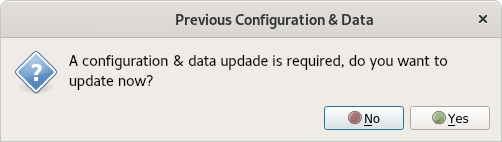
\includegraphics[width=12cm,frame]{../screenshots/config_data_update.png}
  \caption{Configuration and data update}
  \label{fig:db_connect}
\end{figure}

If 'Yes' is selected, the update is performed and the application starts. If 'No' is selected, the application will quit. If previous changes to an outdated configuration are if strong importance, please contact the author for support.

\subsection{Application Startup}
\label{sec:startup}

While ATSDB is more a database framework, it comes with a dedicated client. When the ATSDB client is started a dialog  for opening a database is shown. 

\begin{figure}[H]
  \hspace*{-2cm}
    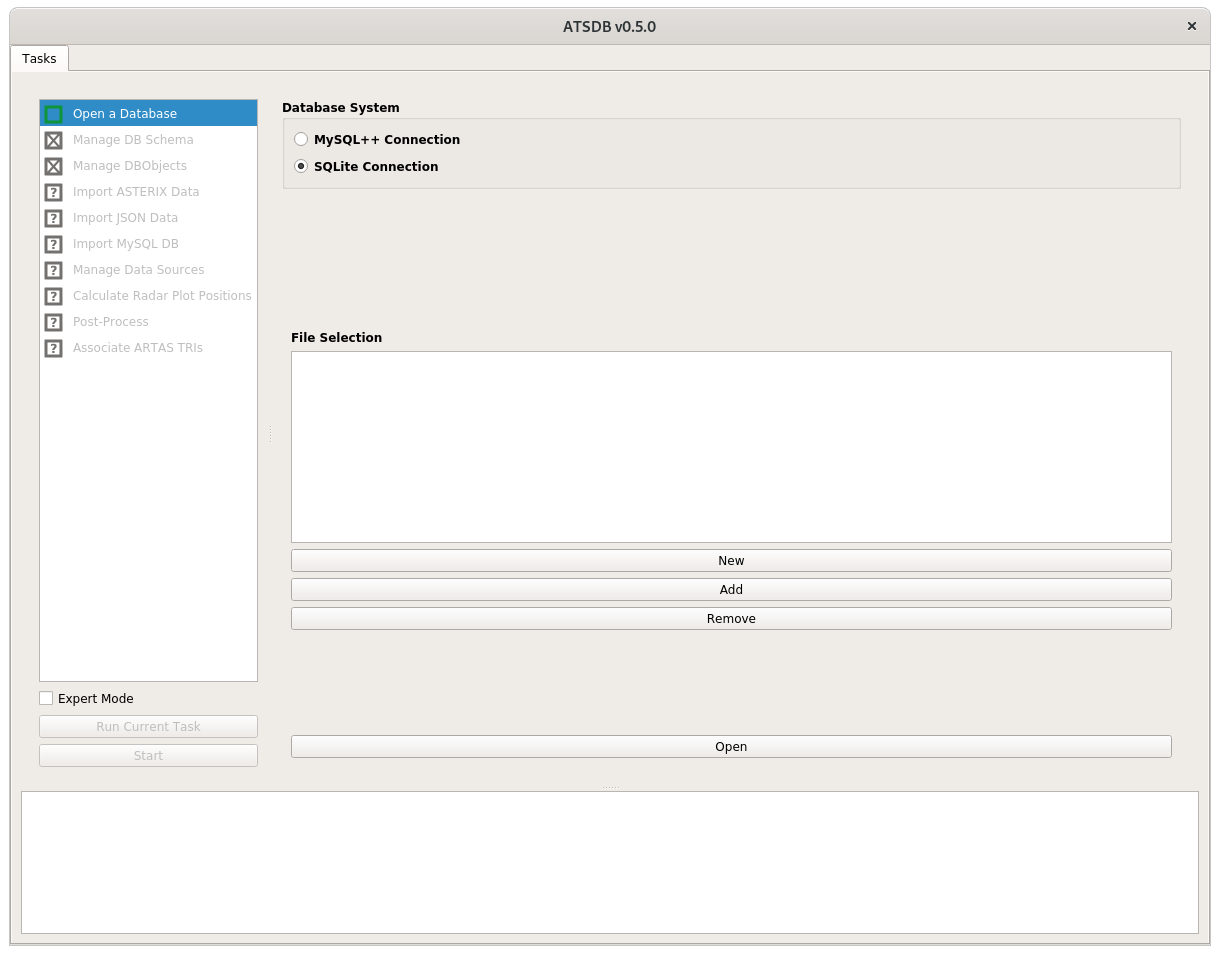
\includegraphics[width=18cm,frame]{../screenshots/db_config_connect.png}
  \caption{Connecting to a database}
  \label{fig:db_connect}
\end{figure}

On the left-hand side, a database system can be selected.  Choices are either MySQL database or a file container with a SQLite3 database. \\
On the lower left (depending on the database system) either a MySQL server connection can be configured or a list of SQLite3 files is shown.\\

On the right-hand side a database schema can be selected and edited (editing is only recommended for experienced users).

\subsection{Connecting to a MySQL Server}

\begin{figure}[H]
  \center
    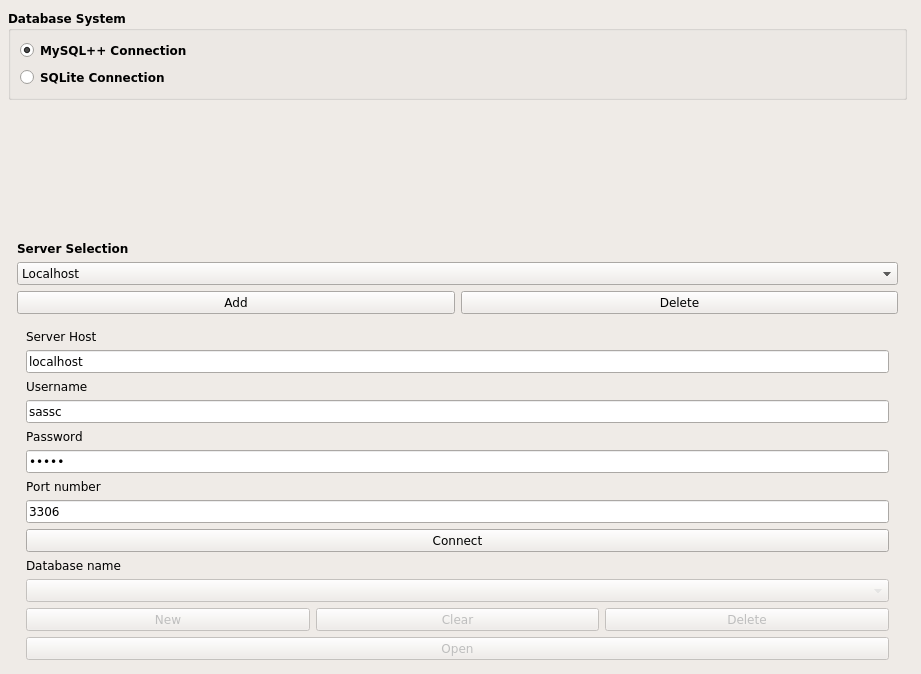
\includegraphics[width=7cm,frame]{../screenshots/mysql_server_selection.png}
  \caption{Connecting to a MySQL server}
  \label{fig:mysql_connect}
\end{figure}

Several MySQL servers can be defined, each one has a specific set of parameters. To add a new server, press the 'Add' button and enter a unique server name. To select the currently used server, use the dropdown menu. To delete the currently used server, press the 'Delete' button.

For connecting to a MySQL database, several parameters have to be entered:

\begin{table}[H]
  \center
  \begin{tabular}{ | l | l | l |}
    \hline
    \textbf{Parameter} & \textbf{Description} & \textbf{Example Values} \\ \hline
    Server Host & Network identifier of server & 'localhost', '10.0.0.123' \\ \hline
    Username & MySQL user name & 'sassc', 'root' \\ \hline
    Password & MySQL user password & 'sassc', '' \\ \hline
    Port Number & MySQL server port & '3306' \\
    \hline
  \end{tabular}
  \caption{MySQL server parameters}
\end{table}

To connect to a defined MySQL server, press the 'Connect' button.\\

\subsubsection{Access to SASS-C MySQL Servers}

Please note that it is not recommended to use SASS-C databases on which actual performance evaluations are to be performed. Using ATSDB, database operations can be performed which might impede results later obtained by using SASS-C. For this reason, it is recommended to either clone an evaluation or use one on which no later SASS-C evaluations are performed.

If a remote server is used, e.g. a SASS-C workstation, remote access might be prohibited, which will result in an access permissions error during connecting. To resolve this, (generally) remote access can be enabled in the servers MySQL configuration. As a superuser, edit the file 'my.cnf', which is commonly found under '/etc/mysql/my.cnf'. 

Find the line that states:
\begin{verbatim}
bind-address = 127.0.0.1
\end{verbatim}

Change the line to:

\begin{verbatim}
#bind-address = 127.0.0.1
\end{verbatim}

Then, restart the MySQL server using one the following commands:

\begin{verbatim}
/etc/init.d/mysqld restart

#OR, depending on your distribution
service mysql restart
\end{verbatim}

Then, to allow access to the databases, log into a MySQL client on the server as root and execute the following commands:

\begin{verbatim}
# log in as root, must be done as superuser
mysql -u root

# grant access rights for your MySQL user, 
# e.g. 'sass', from the your local IP address, 
# e.g. '192.168.0.104', using your password, e.g. 'sassc'
GRANT ALL ON *.* to 'sassc'@'192.168.0.104' IDENTIFIED BY 'sassc';

# set access rights
FLUSH PRIVILEGES;

# exit the MySQL client
exit
\end{verbatim}

After executing these steps once, remote access to this MySQL server from the specified IP address is enabled.

\paragraph{Firewall}

It might also be the case that your installation of SASS-C has an enabled firewall. If that is the case, access to be MySQL ports must be enabled.

\begin{figure}[H]
  \center
    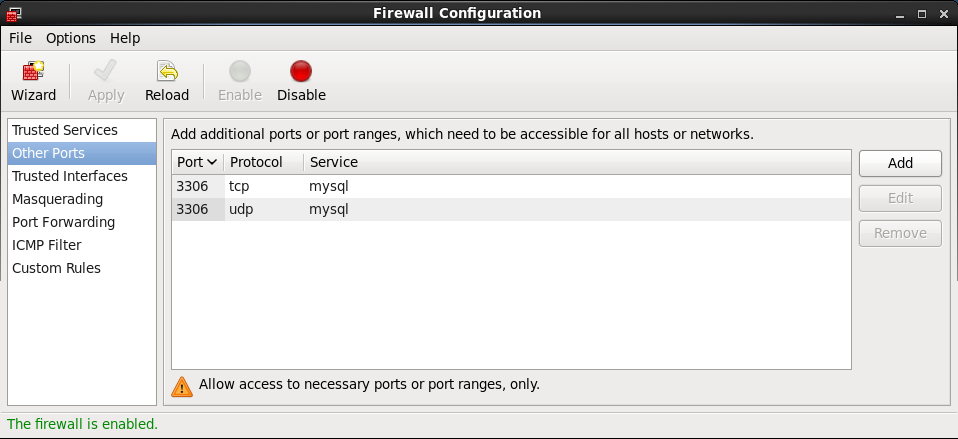
\includegraphics[width=15cm,frame]{../screenshots/centos_firewall.png}
  \caption{MySQL Server firewall example}
\end{figure}

\subsubsection{Error Messages}

If  a  wrong  database  name  or  IP  address  is  used,  error  messages  can  be  e.g.  \\

\begin{figure}[H]
  \center
    \includegraphics[width=9cm,frame]{../screenshots/mysql_connect_error.png}
  \caption{MySQL Server not found error.}
\end{figure}

 or 

\begin{figure}[H]
  \center
    \includegraphics[width=9cm,frame]{../screenshots/mysql_user_error.png}
  \caption{MySQL user incorrect error.}
\end{figure}

If such an error occurs, correcting the server host name and or user/password should solve the problem.

\subsubsection{Opening a MySQL Database}

After successful connection, all existing databases in the server are shown in the 'Database name' drop-down menu. The last used one is selected automatically.

\begin{figure}[H]
  \center
    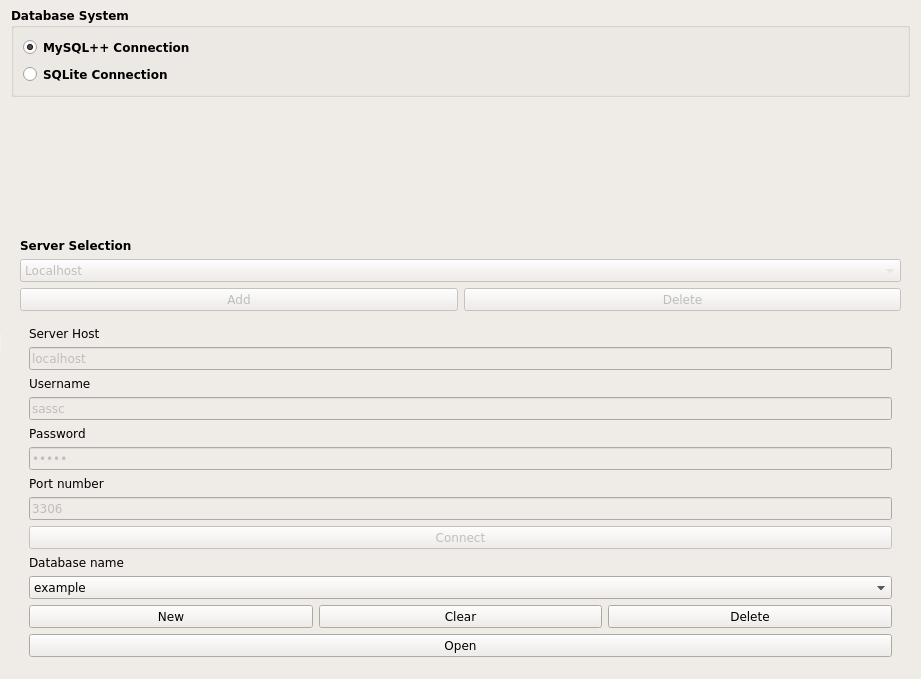
\includegraphics[width=5.5cm,frame]{../screenshots/mysql_database_selection.png}
  \caption{Selecting a MySQL database.}
  \label{fig:mysql_db_select}
\end{figure}

Several actions are available:

\begin{itemize}  
\item Drop-down selection: Selects the current database
\item New button: Allows creation of a new database
\item Clear button: Deletes all data with current database (after confirmation)
\item Delete button: Deletes current database (after confirmation)
\item Open button: Opens the current database
\end{itemize}

\subsubsection{Importing a MySQL Database}

After opening a database, import functions are available by clicking the 'Import' button:

\begin{figure}[H]
  \center
    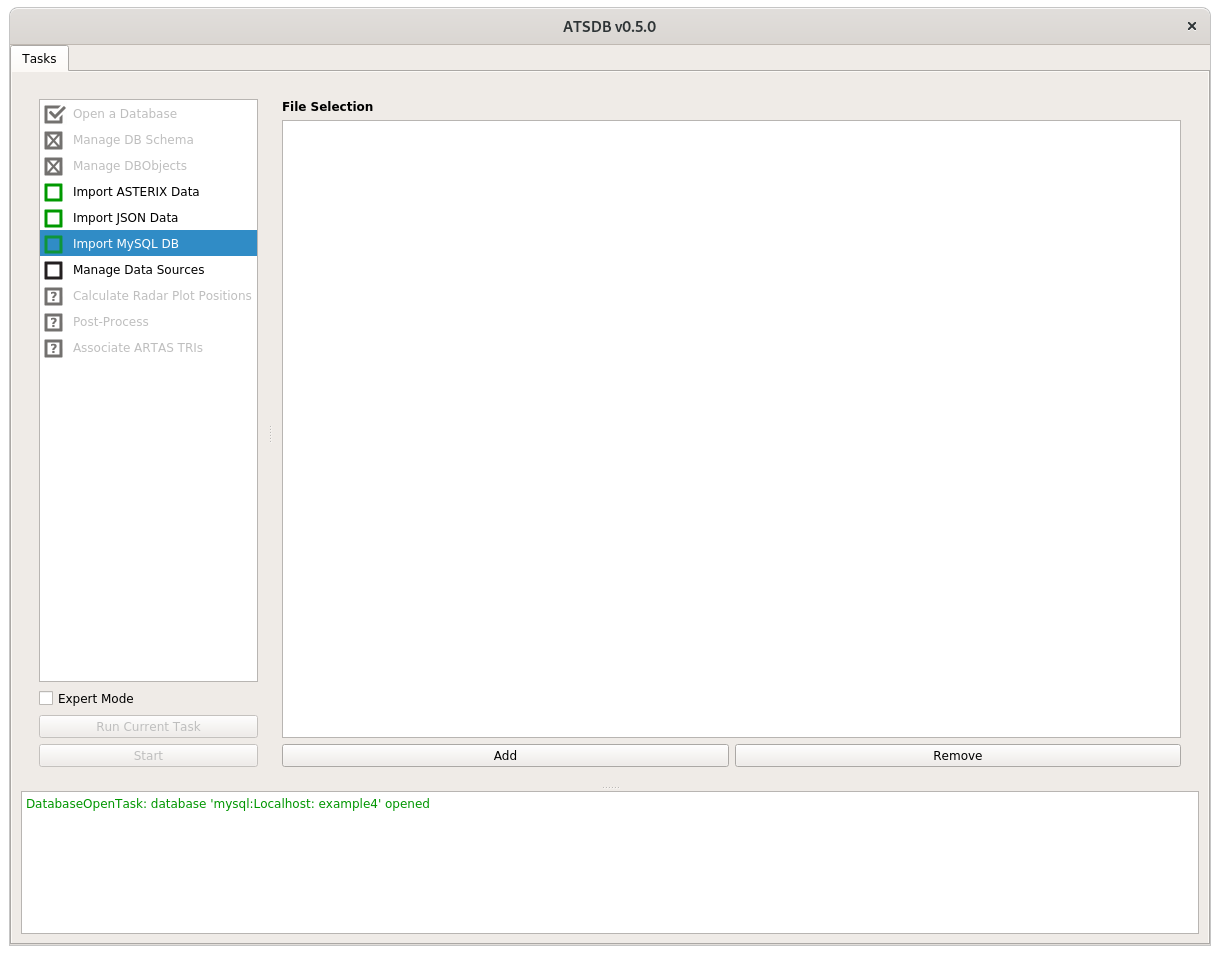
\includegraphics[width=9cm,frame]{../screenshots/database_import.png}
  \caption{Importing a MySQL database}
\end{figure}

\paragraph{Importing a MySQL Text File}

A previously exported MySQL database can be read from a text file and written into the current database. After selecting this option, a file open dialog is shown which allows selection of '*.sql' files. Please note the following points:

\begin{itemize}  
\item The text file must contain valid MySQL statements
\item MySQL functions/views are not imported, only data which can be inspected
\item If more than 3 errors occur during the import process, it is aborted
\item If the import process was aborted, the current database might contain already imported parts which are not deleted automatically
\end{itemize}

\paragraph{Importing a MySQL Text Archive File}

A previously exported MySQL database can be read from a text archive file and written into the current database. After selecting this option, a file open dialog is shown which allows selection of '*.tar.gz *.gz *.tar *.zip *.tgz *.rar' files. Please note the following points:

\begin{itemize}  
\item This function does \textbf{not} work to import an Verif-exported \textit{evaluation tgz}, but imports an \textit{SQL archive} from inside such an evaluation tgz
\item The text archive file must follow the same points as in the \textbf{Importing a MySQL Text File} section.
\item All files within the archive are read and imported into the database
\item If more than 3 errors occur during the import process, it is aborted
\item If the import process was aborted, the current database might contain already imported parts which are not deleted automatically
\end{itemize}

\paragraph{Importing a SASS-C Evaluation Export}

The following steps must be taken:

\begin{itemize}  
\item An export from a SASS-C evaluation must exist, e.g. 'example.tgz'
\item Using your favorite archive manager, extract the file 'tgz-tmp/<JOB\_NAME>/exported.sql.gz'
\item After successfully connecting to a server, create a new database, e.g. '<job\_name>', and open it
\item Click on the 'Import' button and select 'Import MySQL Text Archive File'
\item Select the previously extracted 'exported.sql.gz'
\end{itemize}

\subsection{Opening a SQlite3 File Container}
\label{sec:sqlite_fc}
For opening a file container, three actions are available:

\begin{itemize}  
\item New: Creates a new (empty) SQLite3 container and adds it to the 'File Selection' list
\item Add: Adds an existing  SQLite3 container and adds it to the 'File Selection' list
\item Remove: Removes an entry from the 'File Selection' list
\end{itemize}

After selection of the wanted database container, the 'Open' button can be used for opening the database container.

\begin{figure}[H]
  \center
    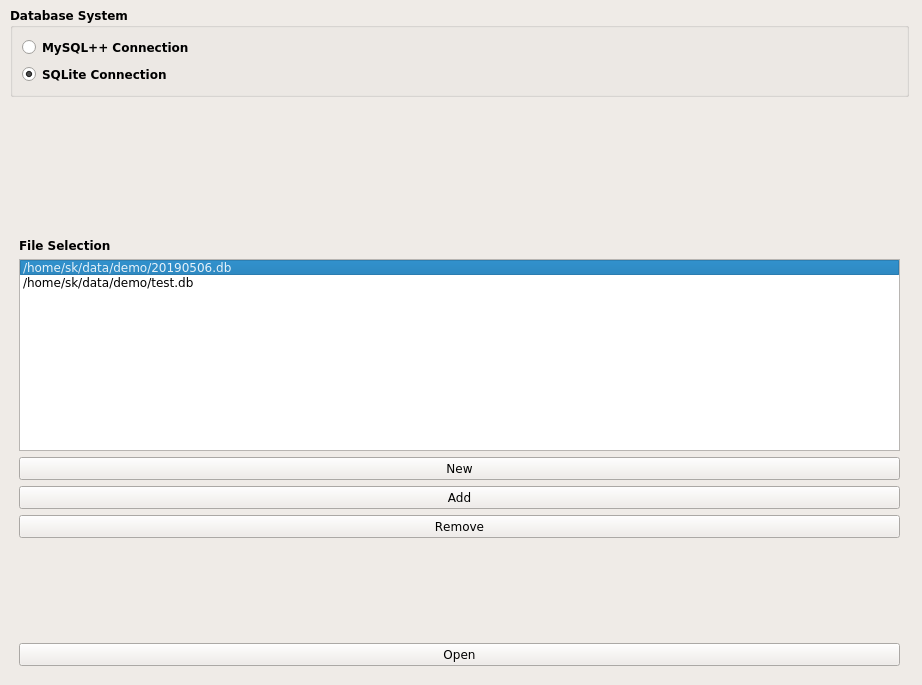
\includegraphics[width=8cm,frame]{../screenshots/sqlite3_open.png}
  \caption{Opening a SQLite3 file container}
  \label{fig:sqlite3_open}
\end{figure}

\subsection{Database Schema Selection}
For a common user, usage of the pre-configured database schema 'SCDB' is recommened. To select a different database schema, please use the 'Schema selection' drop-down menu.\\

\begin{figure}[H]
  \center
    \includegraphics[width=8cm,frame]{../screenshots/database_schema_selection.png}
  \caption{Selecting a database schema}
  \label{fig:db_schema_select}
\end{figure}


\includegraphics[width=0.5cm]{../../data/icons/hint.png} For experienced users, a database schema can be created, edited and selected, which is currently not recommended (since it is not user friendly and might crash if used in the ``wrong'' manner).

\begin{figure}[H]
  \hspace*{-1cm}
    \includegraphics[width=16cm,frame]{../screenshots/database_schema_configuration.png}
  \caption{Configuring a database schema}
  \label{fig:db_schema_configuration}
\end{figure}

\subsection{DBO Management}

Also, after locking the database schema, the existing Database Objects can be edited, which is currently also not recommended, except for editing of data sources. There will be additional information about this subject in a later release, when the functionality has matured.

\subsubsection{Editing of Data Sources}
\label{sec:data_source_editing}

If a database generated by SASS-C is opened, the data sources are already defined. But, if data is imported from JSON, no data source information is given, so this information must either be edited manually, or loaded from a previous SASS-C evaluation. \\

For this purpose, data source information for each DBO can be stored in the configuration, and can be synchronized to/from a database. \\

To edit a data source, lock the schema and press the gear symbol {
\includegraphics[scale=0.02]{../../data/icons/edit.png}.

\begin{figure}[H]
  \hspace*{-1.5cm}
    \includegraphics[width=18cm,frame]{../screenshots/dbo_edit.png}
  \caption{DBO Edit Widget}
  \label{fig:dbo_edit}
\end{figure}

Then, in the top-left corner, press the 'Edit Data Sources' button. If this is done for the first time with an empty database, the widget will look as follows:

\begin{figure}[H]
  \hspace*{-1cm}
    \includegraphics[width=16cm,frame]{../screenshots/dbo_edit_ds.png}
  \caption{DBO Edit Data Sources Widget}
  \label{fig:dbo_edit_ds}
\end{figure}

On the left hand side, the data sources in the configuration are shown and can be edited. A new one can be added using the 'Add New' button, and synchronization to database data sources can be proposed by using the 'Sync to DB' button. \\

In the middle, proposed synchronization are shown. They can be checked, edited or disabled before executing. \\

On the right hand side, the data sources as existing in the currently opened database are shown and can also be edited, as well as synchronized to the configuration. \\

The idea is that all commonly used data sources are defined and persisted in the configuration, and are then used automatically during the JSON import process. \\

Please \textbf{note} that currently the position of data sources is only required for \textbf{Radar} data sources (in the plot position calculation), for the others it would suffice to have SAC/SIC and name information for display purposes.

\paragraph{Editing Database Data Sources}

If SDDL data was imported without stored data source information in the configuration, the widget would look as follows:

\begin{figure}[H]
  \hspace*{-1cm}
    \includegraphics[width=16cm,frame]{../screenshots/dbo_edit_ds_db.png}
  \caption{DBO Edit Data Sources in Database}
  \label{fig:dbo_edit_ds_db}
\end{figure}

The orange fields represent the NULL value, to indicate that this information is not (yet) given. Each of the fields can edited, except for the ID field. \\

In a SASS-C database, all of the values would be set. The same can be achieved by editing. \\

\begin{figure}[H]
  \hspace*{-2cm}
    \includegraphics[width=18cm,frame]{../screenshots/dbo_edit_ds_db2.png}
  \caption{DBO Edit Data Sources in Database Edited}
  \label{fig:dbo_edit_ds_db2}
\end{figure}

\paragraph{Synchchronizing Database Data Sources to Config}

Now, with the already defined data sources, the values should be persisted in the configuration. To achieve this, click on the 'Sync to Config' button to create the proposed actions.

\begin{figure}[H]
  \hspace*{-2cm}
    \includegraphics[width=18cm,frame]{../screenshots/dbo_edit_ds_sync2cfg.png}
  \caption{DBO Edit Synchronize DB Data Sources to Configuration }
  \label{fig:dbo_edit_ds_sync2cfg}
\end{figure}

Since no previous data sources are exist in the configuration, the proposed action is to add all data sources as new ones. Unwanted actions can be disabled with the checkbox or set to 'None' in the drop-down menu. To perform the selected action, click the 'Perform Actions' button.

\begin{figure}[H]
  \hspace*{-2cm}
    \includegraphics[width=18cm,frame]{../screenshots/dbo_edit_ds_db2cfgsynced.png}
  \caption{DBO Edit Synchronized DB Data Sources to Configuration }
  \label{fig:dbo_edit_ds_db2cfgsynced}
\end{figure}

\paragraph{Editing Configuration Data Sources}

The configuration data sources displayed on the left can also be edited, to change names or correct information.

\begin{figure}[H]
  \hspace*{-2cm}
    \includegraphics[width=18cm,frame]{../screenshots/dbo_edit_ds_cfg.png}
  \caption{DBO Edit Data Sources in Configuration}
  \label{fig:dbo_edit_ds_cfg}
\end{figure}

A few values where changed, and the changes will be persisted on correct shutdown of the application.

\paragraph{Synchchronizing Configuration Data Sources to DB}

In the previous step, a few values were changed, and for the data source 'WAM1' the SAC/SIC values were also changed. To synchronize these changes to the currently opened database, click on the 'Sync to DB' button.

\begin{figure}[H]
  \hspace*{-2cm}
    \includegraphics[width=18cm,frame]{../screenshots/dbo_edit_ds_sync2db.png}
  \caption{DBO Edit Synchronize Configuration Data Sources to DB}
  \label{fig:dbo_edit_ds_sync2db}
\end{figure}

Note that the proposed action are to overwrite the data source information for all, except for 'WAM1', where no action is proposed since no matching SAC/SIC could be found. The perform the selected actions, press the 'Perform Actions' button.

\begin{figure}[H]
  \hspace*{-2cm}
    \includegraphics[width=18cm,frame]{../screenshots/dbo_edit_ds_cfg2dbsynced.png}
  \caption{DBO Edit Synchronized Configuration Data Sources to DB}
  \label{fig:dbo_edit_ds_cfg2dbsynced}
\end{figure}


\paragraph{Final Comments}

If the procedure seems complex, please remember that this procedure  has to be performed once for each DBO, after that the data sources are defined in the configuration. Also, if you have access to a SASS-C database, it is easier to synchronize the data source information from there to the configuration. \\

After doing so, for imported JSON the SAC/SIC information supplied in the ASTERIX target reports are used to match them to the respective data source. \\

For matching purposes only the SAC/SIC values are of importance, the name information doesn't have to be unique. If multiple data sources identical SAC/SIC values exist (for whatever reason), the first match is used during import.

\subsection{Tasks}
\label{sec:tasks}

\subsubsection{Importing ASTERIX Data}
\label{sec:asterix_import}

To execute this task select ''Task``->  ''Import ASTERIX Data` in the top menu bar. \\

Please note that the following framings are currently supported:
\begin{itemize}  
\item None: Raw, netto, unframed ASTERIX data blocks
\item IOSS: IOSS Final Format
\item RFF: Comsoft RFF format
\end{itemize}

Please note that the following ASTERIX categories, editions, reserved expansion fields and special purpose fields are currently supported: \\\\

\begin{tabular}{ | l | r | r | r |}
\hline
  CAT & Editions & REFs & SPFs  \\ \hline
  001 & 1.1 &  &  \\ \hline
  002 & 1.0 &  &  \\ \hline
  019 & 1.2, 1.3 & & \\ \hline
  020 & 1.5, 1.8 & 1.3 & \\ \hline
  021 & 2.1 & & \\ \hline
  023 & 1.2 & & \\ \hline
  034 & 1.26 & & \\ \hline
  048 & 1.15 & & \\ \hline
  062 & 1.12, 1.16 & 1.2 & ARTAS TRIs \\ \hline
  063 & 1.0, 1.1 & & \\ \hline
  065 & 1.2, 1.3 & & \\ \hline
\end{tabular} \\

Please note that sensor status messages currently are decoded, but not inserted into the database.

\begin{figure}[H]
  \center
    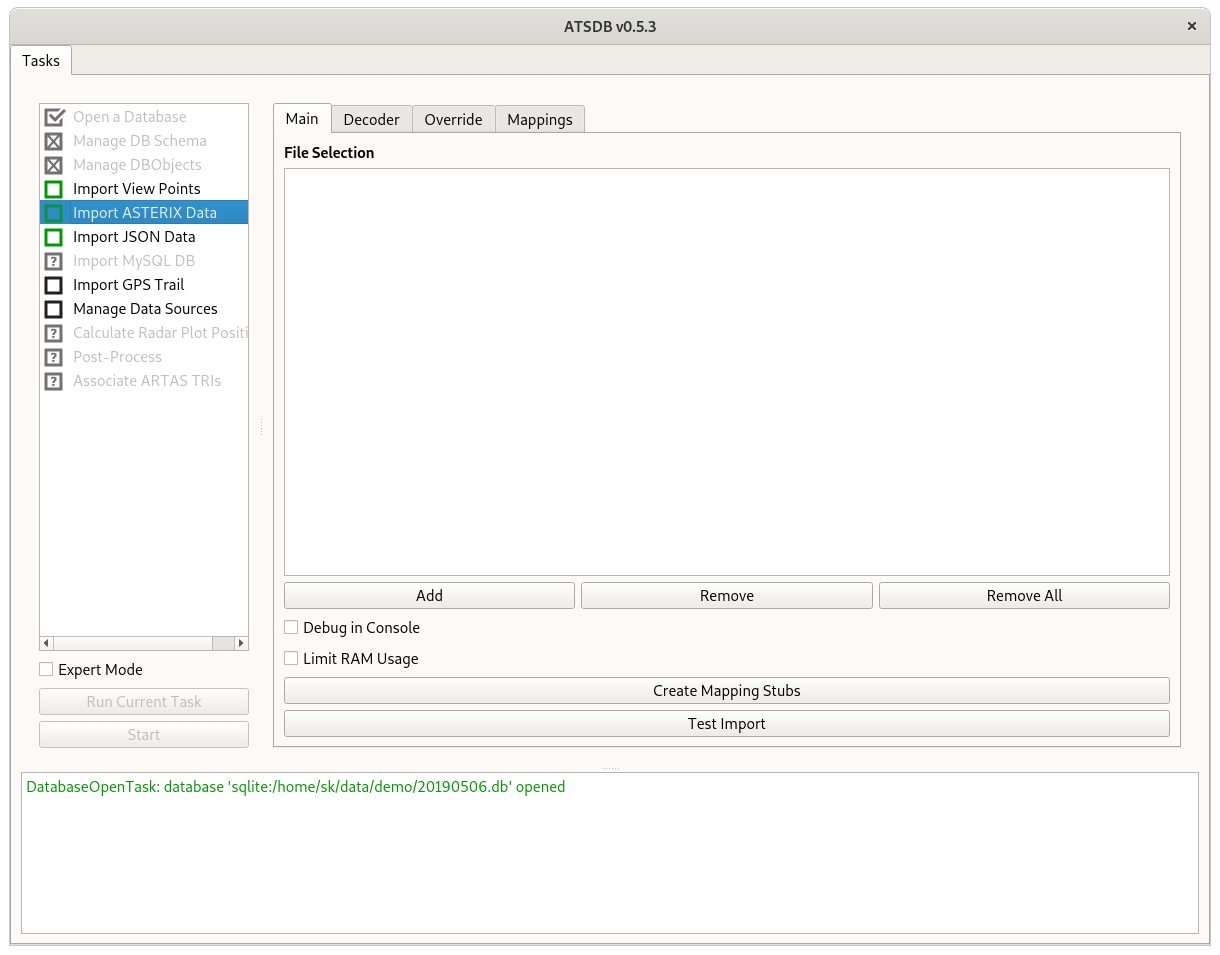
\includegraphics[width=10cm]{../screenshots/asterix_import_data.png}
  \caption{Import ASTERIX Data task}
\end{figure}

In the 'File Selection' list, a list of available ASTERIX data files is given. Entries can be added using the 'Add' button or removed using the 'Remove' buttons. Please add and select the file to be imported.\\

In the 'ASTERIX Configuration' widget the framing, which categories are to be encoded and the currently acitive editions can be set.

Further below, the list of existing JSON object parsers is shown. Each parser parses JSON data and maps to a specific DBO. 

To inspect or edit a JSON object parser, click on it in the list. This step is not required for parsing, but it does give information which ASTERIX content is skipped and which is parsed, and to DBObject variable it is written.

\paragraph{Importing}

Using the 'Debug in Console' checkbox, additional debugging information is output to the console, and the ASTERIX decoding is switched to single-threading for easier investigation.

Using the 'Test Import' button, the import function can be tested without inserting the data into the database, the 'Import' imports the selected file with the given options.

During import a status indication will be shown as follows:

\begin{figure}[H]
  \center
    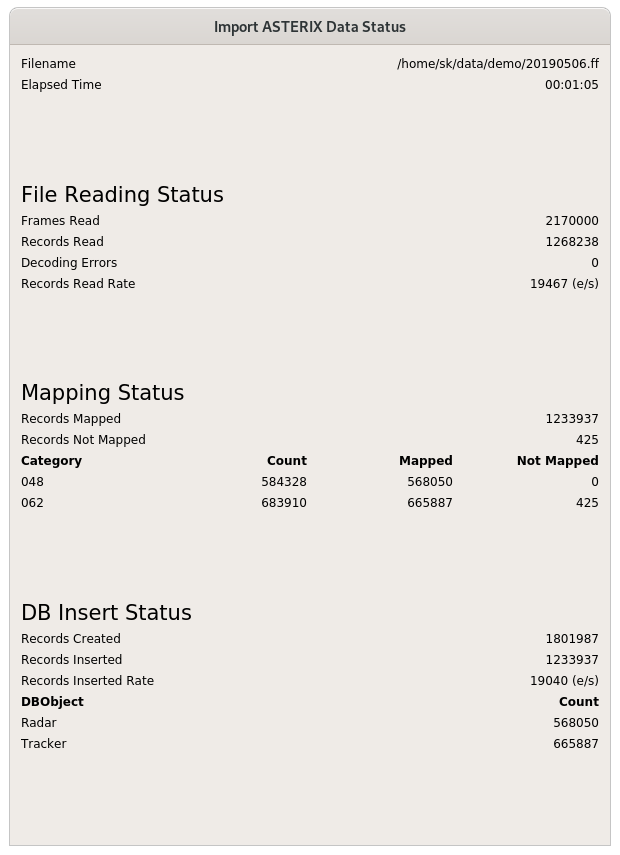
\includegraphics[width=12cm]{../screenshots/asterix_import_status.png}
  \caption{Import ASTERIX data task status}
\end{figure}

If an decoding error occurs, a brief message box is shown, after which the application has to be closed. Please make sure that the correct framing and edition versions are selected, or contact the author for support if this does not resolve the issue.

After import, a confirmation will be shown as follows:

\begin{figure}[H]
  \center
    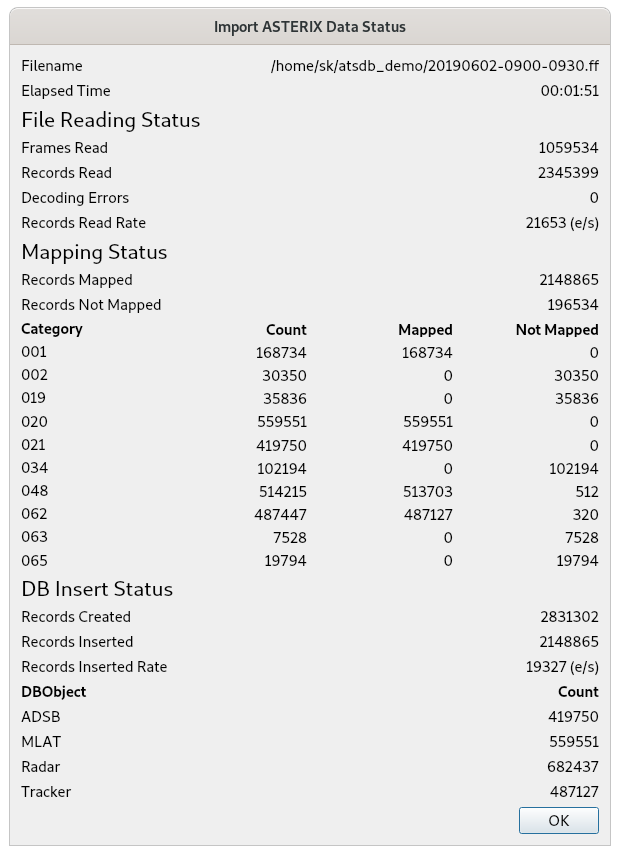
\includegraphics[width=10cm]{../screenshots/asterix_import_done.png}
  \caption{Import ASTERIX data task done}
\end{figure}

Importing performance strongly depends on CPU performance (multi-threading very beneficial), but a import of 2.8 million target reports takes about 2 minutes on the author's hardware. \\


\includegraphics[width=0.5cm]{../../data/icons/hint.png} Please also note that an import can only be performed once, after that the application has to be closed and started again if additional ASTERIX importing is wanted. \\


\includegraphics[width=0.5cm]{../../data/icons/hint.png} Please also note the currently not all data fields (as shown in the JSON object parsers) are imported.\\

The (truncated) timestamps of CAT001 are calculated in a simple algorithm based on the CAT002 messages from the same sensor. \\\\


\includegraphics[width=0.5cm]{../../data/icons/hint.png} After the import it is recommended to re-start the application, since currently a memory leak during import exists. While this does not affect the import process, usage of the application directly after the import process will be slower than usual. A re-start of the application resolves this issue. This will be fixed in the next version. \\

\subsubsection{Importing JSON Data}
\label{sec:json_import}

For information about test dataset please refer to \nameref{sec:test_data}. \\

To execute this task select ''Task``->  ''Import JSON Data` in the top menu bar.

\begin{figure}[H]
  \center
    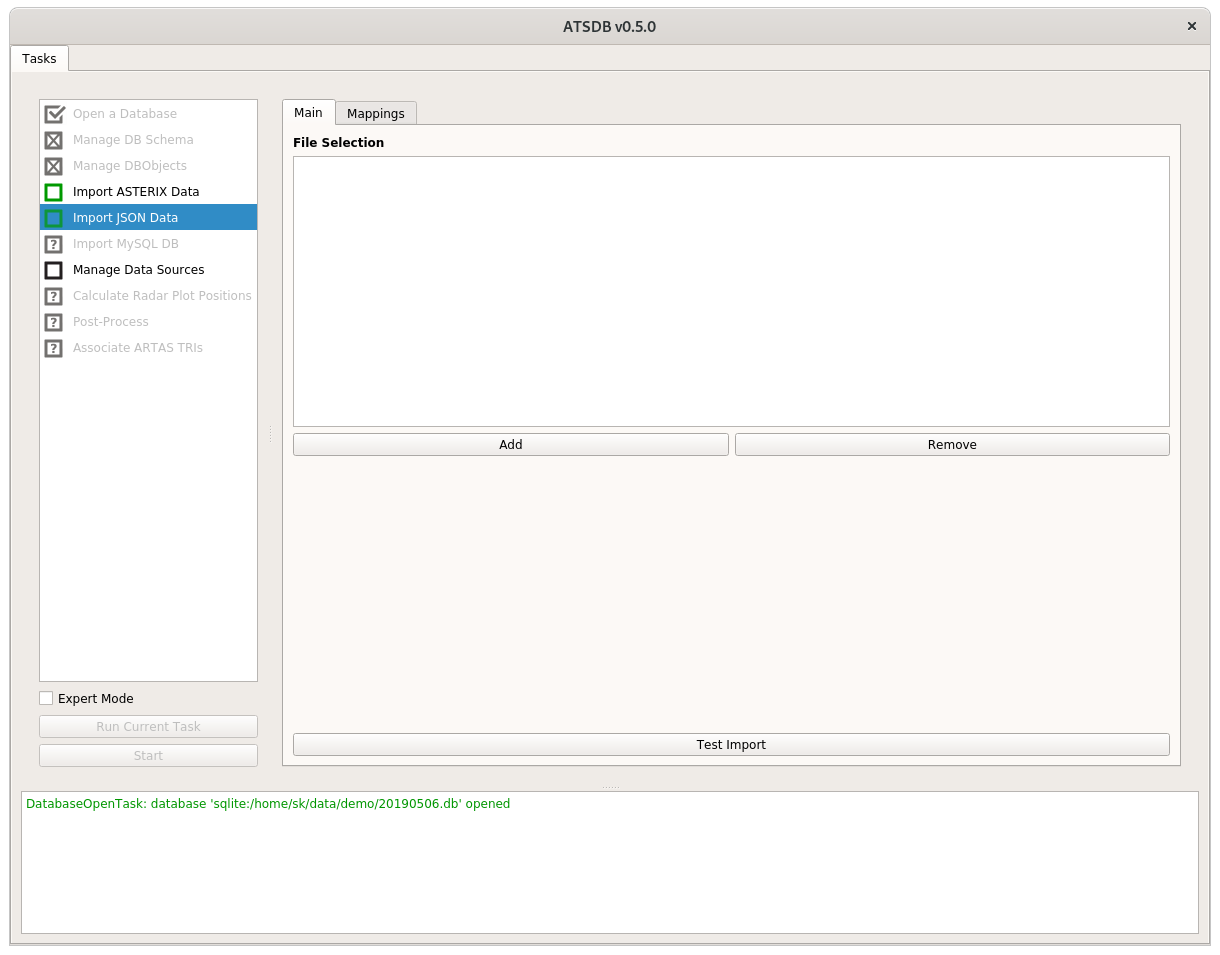
\includegraphics[width=14cm,frame]{../screenshots/import_json_data.png}
  \caption{Import JSON Data task}
\end{figure}

In the 'File Selection' list, a list of available JSON data files is given. Entries can be added using the 'Add' button or removed using the 'Remove' buttons. Please note that either native JSON text files can be imported, or archives containing the same with the following formats: *.zip, *.gz, *.tgz \\

Below, the JSON parsing schema can be selected, the following options exist:
\begin{itemize}  
\item SDDL: Import JSON created by the SDDL v0.2 tool
\item ADSBexchange: Import JSON from the ADSBexchange platform
\item OpenSkyNetwork: Import JSON from the OpenSky Network platform
\end{itemize}

A new schema can be added using the ``Add'' button, or an existing removed using the ``Remove'' button. \\

Further below, for the selected parsing schema, the list of existing JSON object parsers is shown. Each parser is specialized for a specific DBO, in the shown example of OpenSkyNetwork, only ADSB exists, since no other data is provdided. \\

To inspect or edit a JSON object parser, click on it in the list. This step is not required for parsing.

\begin{figure}[H]
  \hspace*{-1cm}
    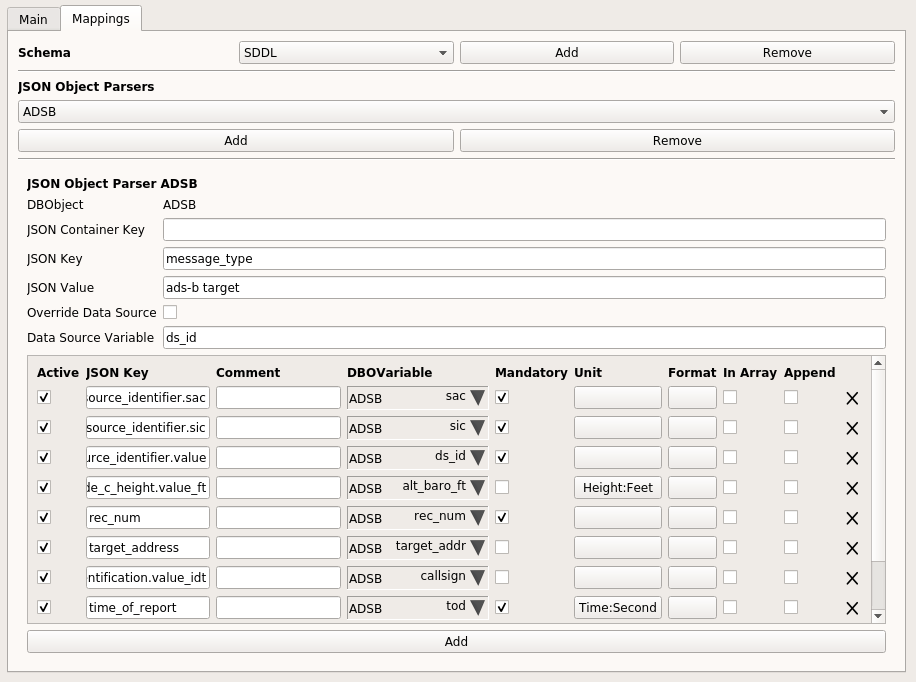
\includegraphics[width=16cm,frame]{../screenshots/import_json_data_object_parser.png}
  \caption{Import JSON Data Object Parser}
\end{figure}

If selected, on the right hand side shows a configuration widget for the selected parser.

\paragraph{JSON Object Parser Configuration}
At the top, a number of configuration options are given:

\begin{itemize}  
\item JSON Container Key: JSON key identifier where nested target reports are stored
\item JSON Key: JSON key identifier for selective parsing
\item JSON Value: JSON value for selective parsing
\item Override Data Source: Checkbox to specify if data source value should be overridden
\item Data Source Variable: Data source variable, for if data source value should be overridden
\end{itemize}


Below list of JSON to DBO variable mappings, with the following options:

\begin{itemize}  
\item Active: Checkbox if mapping should be used for import, mandatory ones must be active
\item JSON key: JSON key identifier
\item DBOVariable: DBO variable that data is mapped to
\item Mandatory: Sets if JSON key/value have to be present, otherwise the JSON object is skipped
\item Unit: Unit of the JSON value
\item Format: Parsing specialization for JSON value
\end{itemize}

A new mapping can be added using the ``Add'' button.

\paragraph{Importing}
Using the 'Test Import' button, the import function can be tested without inserting the data into the database, the 'Import' imports the selected file with the given options.

During import a status indication will be shown as follows:

\begin{figure}[H]
  \center
    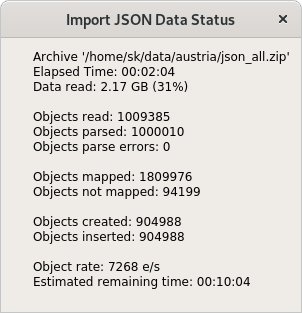
\includegraphics[width=9cm,frame]{../screenshots/json_import_status.png}
  \caption{Import JSON data task status}
\end{figure}

If datasizes can be read from the archive (supported by ZIP but not by GZIP), predictions about the remaining time will be shown.

After import, a confirmation will be shown as follows:

\begin{figure}[H]
  \center
    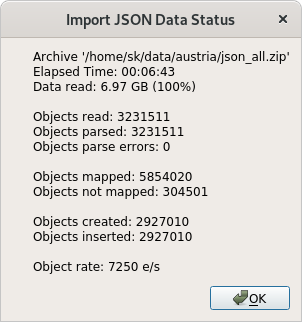
\includegraphics[width=9cm,frame]{../screenshots/json_import_done.png}
  \caption{Import JSON data task done}
\end{figure}

Importing performance strongly depends on CPU performance (multi-threading very beneficial), but a SDDL JSON import of 2.5 million target reports takes about 7 minutes on the author's hardware. \\


\includegraphics[width=0.5cm]{../../data/icons/hint.png} Please note that, since ADSBexchange JSON is not compliant to JSON standard (at least from the used test datasets), parsing errors will be shown and only a small percentage of target reports is imported. This will be improved in the near future.\\

\subsubsection{Calculate Radar Plot Position}

Please note that if no Radar target reports exist in the database, this steps does not have to be performed.\\

Since in SASS-C Verif radar plot coordinates are not given as latitude/longitude, which are the main coordinates for all processing in ATSDB, optionally these coordinates can be re-calculated and set in the database using the ''Calculate Radar Plot Position`` Task. \\

To execute this task select 'Task'->  'Calculate Radar Plot Position' in the top menu bar. \\

Please note that for this step the data source positions have to set in the database, otherwise no plot position can be calculated. If a database generated by SASS-C is used, this should already be the case. For ones created by SDDL JSON, the steps described in \nameref{sec:data_source_editing} have to be performed once.

\begin{figure}[H]
  \center
    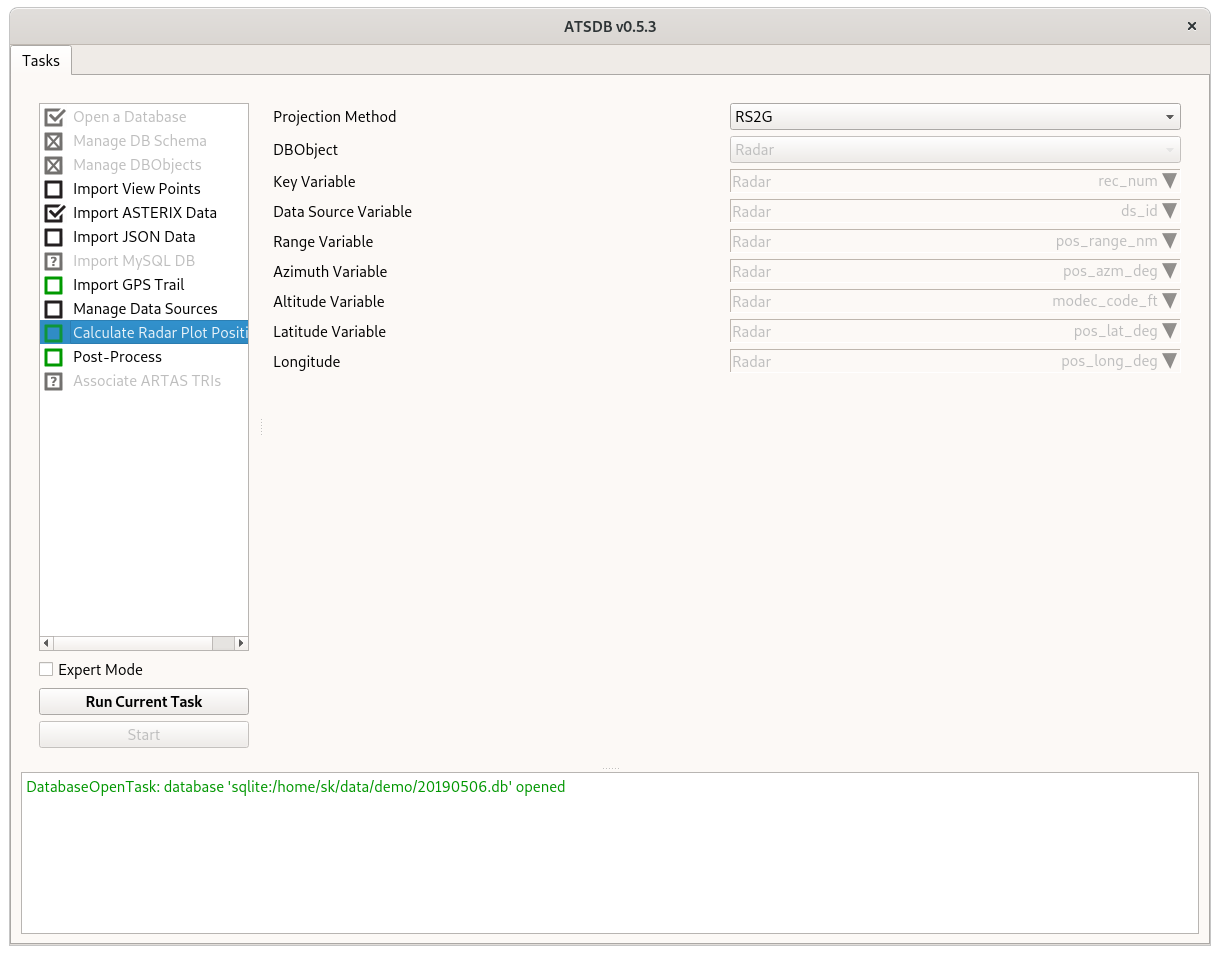
\includegraphics[width=14cm,frame]{../screenshots/task_calc_radar.png}
  \caption{Calculate radar plot position task}
  \label{fig:task_calc_radar}
\end{figure}

There are two projection methods (radar polar coordinates to WGS-84 coordinates) available. The \textit{RS2G} projection is the currently recommended option.

\paragraph{OGR Projection}

The EPSG code for the projection has to be chosen according to your needs, please refer to \url{http://spatialreference.org/ref/epsg/} for a list of possible codes.

The WGS84 latitude/longitude coordinates are then calculated using the radar positions in the database, the range and the azimuth. Please \textbf{note} that currently there will be offsets in the projected coordinates compared to the e.g. the ARTAS projection. The reason for this is under investigation.

\paragraph{RS2G Projection}

For this projection, no additional attributes must be given. Please \textbf{note} that this projection is based on a common 'radar slant to geodesic transformation', it should be equvalent to the ARTAS projection. A verification is still needed, please contact the author if you would be willing to support this.

\paragraph{Calculation}

Press 'Calculate' to start the calculation process, which will take a few minutes depending on the data size. \\

Messages like these will be printed in the text console, the last one indicates completion of the task:

The following windows will be shown, to give indication about the calculation progress:

\begin{figure}[H]
  \center
    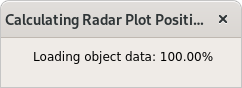
\includegraphics[width=4cm,frame]{../screenshots/task_calc_radar_load.png}
  \caption{Calculate radar plot position task: Loading}
\end{figure}

\begin{figure}[H]
  \center
    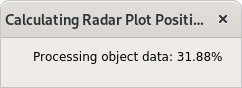
\includegraphics[width=4cm,frame]{../screenshots/task_calc_radar_process.png}
  \caption{Calculate radar plot position task: Processing}
\end{figure}

If there were projection errors in the calculation, the before insertion the user will be asked to confirm. The coordinates with projection errors will of course not be committed to the database, but will be skipped.

\begin{figure}[H]
  \center
    \includegraphics[width=9cm,frame]{../screenshots/task_calc_radar_insert.png}
  \caption{Calculate radar plot position task: Insertion question on errors}
\end{figure}


\begin{figure}[H]
  \center
    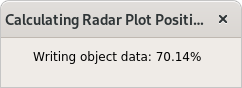
\includegraphics[width=4cm,frame]{../screenshots/task_calc_radar_write.png}
  \caption{Calculate radar plot position task: Writing}
\end{figure}

\begin{figure}[H]
  \center
    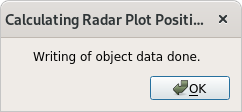
\includegraphics[width=8cm,frame]{../screenshots/task_calc_radar_done.png}
  \caption{Calculate radar plot position task: Done}
\end{figure}

After running this task once (per database), the radar plots also have a set latitude/longitude. As stated, a post-processing step is recommended after executing this task. \\

Please \textbf{note} that this task can be re-run with different projections if wanted.

Please \textbf{note} that no additional Radar plot information is changed, only the latitude/longitude variables are updated.

\subsubsection{Calculate ARTAS Associations Information}

Please note that if no ARTAS TRI SPF information exists in the database, this steps does not have to be performed.\\

\begin{figure}[H]
  \center
    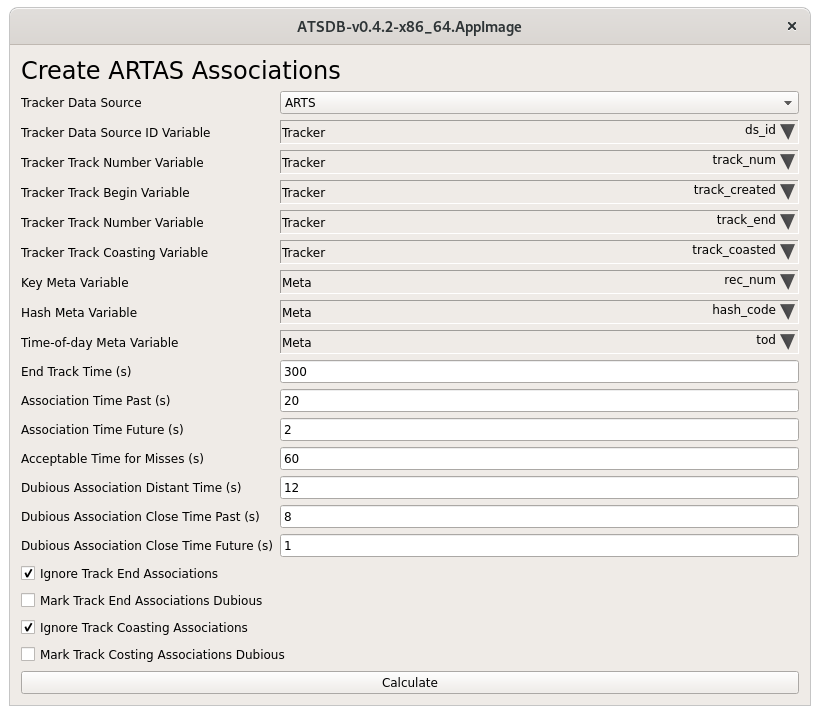
\includegraphics[width=12cm]{../screenshots/artas_association_config.png}
  \caption{Calculate ARTAS associations task: Configuration}
\end{figure}

In this task, the ARTAS association information stored in system track updates can be used to create UTN which associate each system track update to the used sensor target reports.

The following configuration options exist

\begin{itemize}  
\item Tracker Data Source: Name of tracker data source from which associations shall be created.
\item Data Variables: Definition of variables to be used in processing. Does not have to be changed.
\item End Track Time (s): Track update gap time (in seconds) after which a new UTN will be created (even if no track begin/end flag is set).
\item Association Time Past (s): Time window length (in seconds) into the past where sensor target reports are considered for association.
\item Association Time Future (s): Time window length (in seconds) into the future where sensor target reports are considered for association.
\item Acceptable Time for Misses (s): Time window length at the beginning and end of the recording (in seconds) where misses (not found hash codes) are acceptable.
\item Dubious Association Distant Time (s): Maximum age of made associations (in seconds), if older they are considered as dubious associations.
\item Dubious Association Close Time Past (s): Time window length (in seconds) into the past where made associations are considered as dubious if multiple sensor hashes exist.
\item Dubious Association Close Time Future (s): Time window length (in seconds) into the future where made associations are considered as dubious if multiple sensor hashes exist.
\item Ignore Track End Associations: If set, no assocations for system track updates where the track end flag is set are created.
\item Mark Track End Associations Dubious: If set, assocations for system track updates where the track end flag is set are counted as dubious.
\item Ignore Track Coasting Associations: If set, no assocations for system track updates where the track coasted flag is set are created.
\item Mark Track Coasting Associations Dubious: If set, assocations for system track updates where the track coasted flag is set are counted as dubious.
\end{itemize}

\paragraph{UTN Creation from System Track Numbers and End Track Time}: 

The task should create a unique target number (UTN) for every ARTAS track. The track begin/end flags therefore are used to create new UTNs or finalize existing ones. To cover the case when such information is wrong or missing, the 'End Track Time' is used to check the time between track updates from one track number. If the gap is larger then the defined time, a new UTN is created even if no track begin/end flag was set.

\paragraph{Association Time Window}

Consider the following figure: In a timeline, a system track update exists at time \textbf{0}, while referenced sensor target reports exist at the times \textbf{1,2,3}.


\begin{figure}[H]
  \center
    
\includegraphics[width=12cm]{../screenshots/artas_assoc_timeline.png}
\end{figure}


The time window defined by [\textit{Association Time Past, Association Time Future}] defines which referenced sensor target reports are considered for association. In this case, 1 and 2 are considered, while 3 is disregarded. Since 1 is closer in time to the system track update, the association between (0,1) is made.

\begin{figure}[H]
  \center
    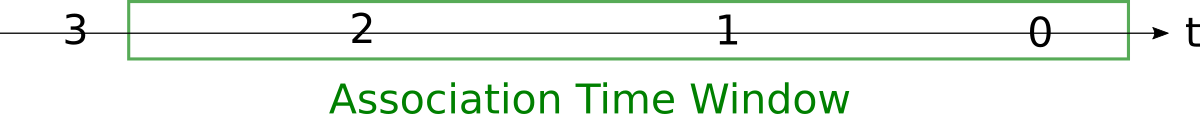
\includegraphics[width=12cm]{../screenshots/artas_assoc_window.png}
\end{figure}

The time defined by \textit{Dubious Association Distant Time} is used to mark assocations which are older than the defined time as dubious. The associations are still created, but counted as dubious. Since 2 is still in the association time window, the assocation (0,2) is made but counted as dubious.

\begin{figure}[H]
  \center
    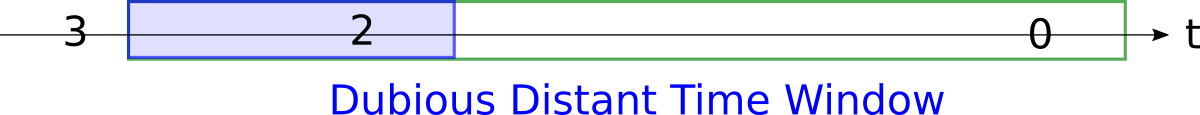
\includegraphics[width=12cm]{../screenshots/artas_assoc_dubious_distant_window.png}
\end{figure}


The time window defined by [\textit{Dubious Association Close Time Past, Dubious Association Close Time Future}] defines when assocations are counted as dubious if multiple referenced sensor target reports exist in it. In this case, 1 and 2 are considered for association, and since 1 is closer in time to the system track update, the association between (0,1) is made. But, since 2 also falls into this time window, the association of (0,1) is counted as dubious association.

\begin{figure}[H]
  \center
    
\includegraphics[width=12cm]{../screenshots/artas_assoc_dubious_close_window.png}
\end{figure}

\begin{figure}[H]
  \center
    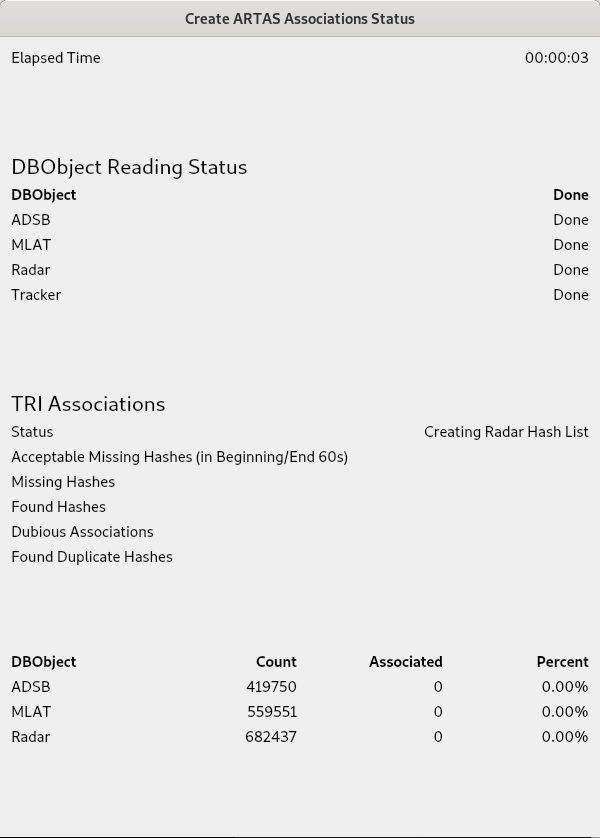
\includegraphics[width=10cm,frame]{../screenshots/artas_assoc_status.png}
  \caption{Calculate ARTAS associations task: Status}
\end{figure}

\begin{figure}[H]
  \center
    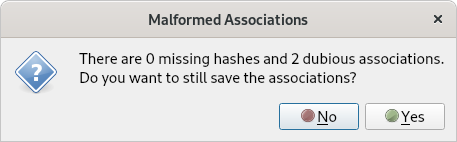
\includegraphics[width=8cm]{../screenshots/artas_assoc_question.png}
  \caption{Calculate ARTAS associations task: Save question}
\end{figure}


\begin{figure}[H]
  \center
    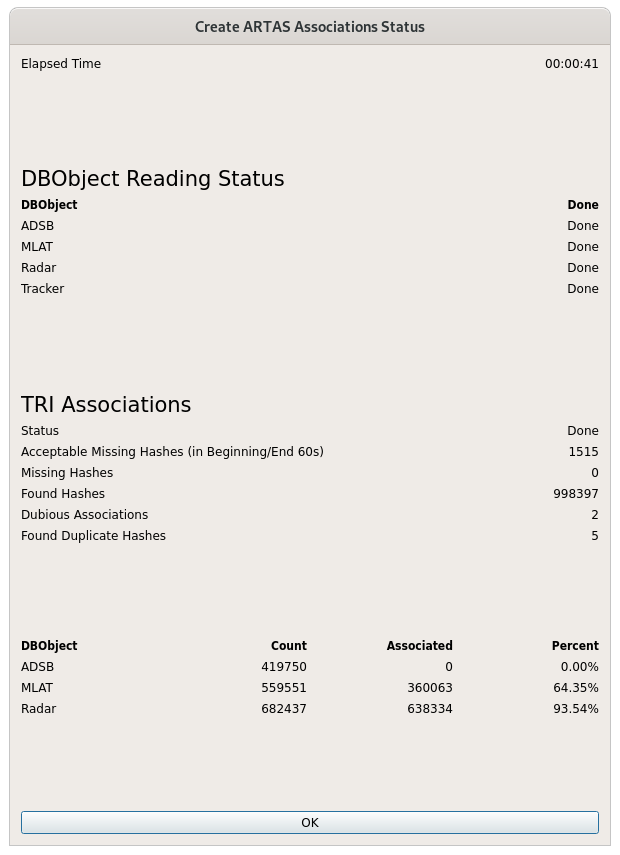
\includegraphics[width=10cm]{../screenshots/artas_assoc_done.png}
  \caption{Calculate ARTAS associations task: Done}
\end{figure}

\subsection{Starting}

After the previous steps have been completed, the 'Start' button can be pressed to continue. \\

\begin{figure}[H]
  \center
    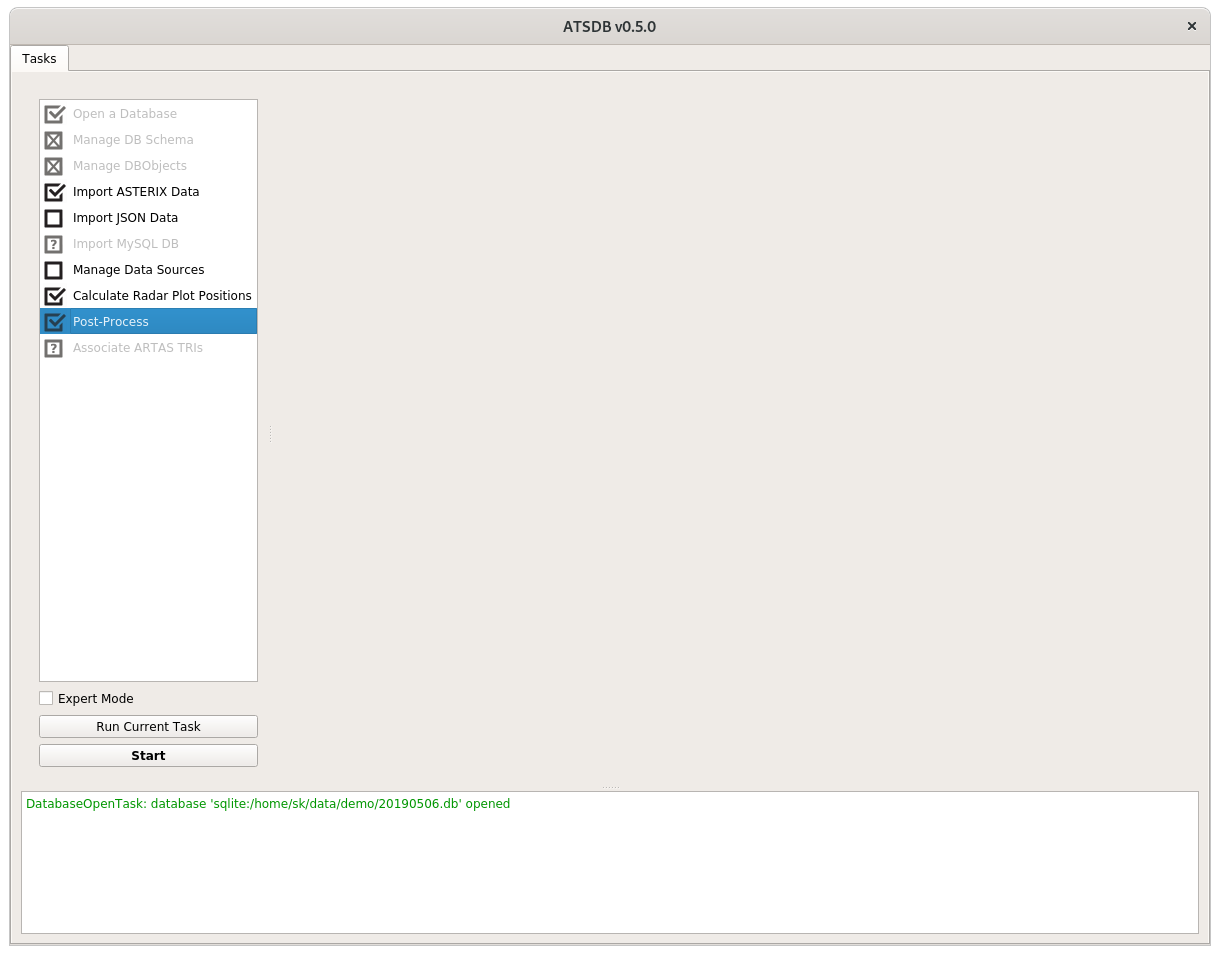
\includegraphics[width=9cm,frame]{../screenshots/start.png}
  \caption{Starting}
\end{figure}

When a database is opened the first time, a post-processing will be performed automatically.

\subsubsection{Postprocessing}
When a database is imported, some information that eases usage of the software does not exist. This information is generated once during a post-processing step, which is automatically performed the first opening of a new database. If wanted, it can always performed using the 'Force post-processing' checkbox.

\begin{figure}[H]
  \hspace*{-2cm}
    \includegraphics[width=18cm,frame]{../screenshots/db_postprocessing.png}
  \caption{Post-processing a database}
  \label{fig:db_postprocessing}
\end{figure}

The following information is generated and stored in the database:

\begin{itemize}  
\item List of all active data sources for all DBOs
\item List with all minima/maxima for all variables of all DBOs
\end{itemize}

This step has to be performed only once for each database, and may take up to a few minutes for large datasets. \\

\includegraphics[width=0.5cm]{../../data/icons/hint.png} Please \textbf{note} that during this step, no DBO data itself is changed, but only additional information is generated and stored in separate database tables.
 

\section{Management}
\label{sec:management}

After pressing the 'Start' button, a management window is shown.

\begin{figure}[H]
  \hspace*{-2cm}
    \includegraphics[width=18cm,frame]{../screenshots/management.png}
  \caption{Main management window}
  \label{fig:management}
\end{figure}

In the uppermost part, the current tab can be selected. The following tabs exist:

\begin{table}[h]
  \center
  \begin{tabular}{ | l | l |}
    \hline
    \textbf{Tab} & \textbf{Description} \\ \hline
    DB Config & Database configuration, used during startup \\ \hline
    Management & All elements to manage loading and inspection of data \\ \hline
    ... & Additional tabs with Views \\
    \hline
  \end{tabular}
  \caption{Main window tab list}
\end{table}

Located in the main window, a management tab exists.  It shows general database information, a list of database objects with loading functions, a filter system and so on.

\subsection{Database Information}

In this widget, general information about the database is given. 

\begin{figure}[H]
  \center
    \includegraphics[width=8cm,frame]{../screenshots/management_database.png}
  \caption{Management: Database Information}
  \label{fig:management_database}
\end{figure}

This also includes the database status.

\subsection{Database Objects}
\label{sec:management_dbos}

In this widget, information about the DBO's, the loaded dataset, and the loading parameters are given.

\begin{figure}[H]
  \center
    \includegraphics[width=8cm,frame]{../screenshots/management_dbos.png}
  \caption{Management: Database Objects}
  \label{fig:management_objects}
\end{figure}

Each existing DBO is listed, and active ones have the following items:

\begin{itemize}
 \item Name checkbox: Defines whether data from this DBO should be loaded
 \item Loading status information
  \begin{itemize}
  \item Idle: Nothing to do at the moment
  \item Loading: DBO read/write in progress
  \end{itemize}
 \item Loaded data size: Number of loaded items / Number of existing items
\end{itemize}

If a DBO exists, but has no data in the database, it is shown as inactive (greyed out, like ADSB in the screenshot).\\

The following important elements exits:
\begin{itemize}
 \item 'Associations' label: Indicates if association information exists, and from which data source
 \item 'Use Filters' checkbox: Whether filtering should be performed
\end{itemize}


Additionally, parameters which configure the loading process exist:

\begin{itemize}
 \item 'Use order' checkbox: Whether the dataset should be ordered by a DBO variable
 \item 'Use Ascending' checkbox: If ordered, defines if it should be ascending or descending
 \item 'Order Variable' selection: If ordered, what variable should be used
 \item 'Use Limit' checkbox: If the data size should be limited
 \item 'Limit Min': If limited, the data set will start at the n-th index given here. If 0, it will be loaded from the beginning, if e.g. 100, the first 100 entries will be skipped and the 101st entry will be the first in the dataset.
\item 'Limit Max': If limited, the number given here will be the number of loaded entries.
\end{itemize}

Using the ``Load'' button , a loading process using the current configuration is started. When a loading process is in progress, the button displays ``Stop'' and can be used to abort the current loading process. Please note that aborting can take a few seconds during which the button is inactive, after successful abort the button states ``Load'' and is usable again.

\subsection{Filters}

\begin{figure}[H]
  \center
    \includegraphics[width=7cm,frame]{../screenshots/management_filters.png}
  \caption{Management: Filters}
  \label{fig:management_filters}
\end{figure}

Each filter consists of a checkbox, defining if a filter is active (contributes to the search query), a triangle-button (to show/hide the filter configuration elements), a unique name, and a manage button (activates a context menu). At the bottom an 'Add filter' button exists, which can be used to add new filters. \\

Please \textbf{note} that the filter configuration will be saved at program shutdown, which is also true for new
filters.   At  startup,  all  filters  from  the  configuration  are  generated  and  restored  to  their  previous  state. However, when the database was changed (usage of different data source), all filters are reset to an initial
state (since their previous configuration may be senseless). \\

Please also \textbf{note} that active filters, at the moment, are always combined with a logical AND. Therefore,
when  two  filters  are  active,  only  the  intersection  of  data  which  both  filters  allow  is  loaded.   A  logical combination of filters using an OR operation is planned, but was not implemented yet.

\subsubsection{Data Source Filters}
For each DBO with a data sources list, a data source filter is generated which can not be edited or deleted.  For each
data source a checkbox exists, which is only active if the data source was active in the database. If checked, the
data generated by the data source is loaded, and otherwise not.

\subsubsection{Custom filters}
A  custom  filter  does  not  differ  in  general  usage,  but  the  inner  workings  are  different.   Also,  it  can  be generated using the 'Add filter' button. It can also be reset (to the original values) edited and deleted using
the manage button. \\
A custom filter consists of one or more filter conditions.  Such a condition involves a DBO (or meta) variable, an operator, and a value.  When active, the filter restricts all loaded DBO data to be fullfill all filter conditions.
As an example, the ``Time of Day'' filter limits the loaded data to a specific time window, to load only time slices of the dataset.  The ``Mode 3A Codes`` filter restricts to a list of (comma-separated) Mode 3/A codes, to single out specific flights. \\

For more information about filtering, please refer to Section \nameref{sec:filtering}.

\subsection{Views}

\begin{figure}[H]
  \center
    \includegraphics[width=8cm,frame]{../screenshots/management_views.png}
  \caption{Management: Views}
  \label{fig:management_views}
\end{figure}

This element allows generation and management of all active Views and windows. Each View is contained
in a tab within a parent window.  At startup, only the main window exists ('MainWindow'), which also holds
the management tab. If the main window is closed, the ATSDB client shuts down. New Views can be added using the 'Add View' button, which opens a pull-down menu. Each View can either be added to the main window ('MainWindow') or into a new window. When added, a new tab exists in the containing window, and controlling elements are added for any new
windows or views. \\

Currently, only the Listbox View exist, for more information about this View, please refer to Section \nameref{sec:listbox_view}.\\

New Views can be added either to currently existing windows as new tabs, or to a newly opened window. A window can be closed either by the close button in the window decoration, which discards all contained Views within the window.  To delete a single View, one can use the close button in the GUI, which frees up all its allocated resources. Each View adds its required variables to the loading list for the database.  During a loading process, the loading status  of a View is shown in the management tab.\\

For more information about Views, please refer to Section \nameref{sec:inspection}.

\subsection{Jobs}

The ATSDB framework supports multi-threading. A number of processing steps (''Jobs``) can be exectuted on a number of parallel threads. Since multi-threading on a database creates limited benefit, only one thread is used specifically for database jobs. All non-database jobs are exectuted on a dynamic number of other threads, which are increased/decreased in number depending on the application's needs. 

\begin{figure}[H]
  \center
    \includegraphics[width=8cm,frame]{../screenshots/management_jobs.png}
  \caption{Management: Jobs}
  \label{fig:management_jobs}
\end{figure}

In the Job element the number of database jobs is listed under ''DB Jobs``, the number of other Jobs is listed under ''Jobs``. The number of active processing threads is listed under ''Threads``.
 

\section{Filtering}
\label{sec:filtering}

\begin{figure}[H]
  \center
    \includegraphics[width=8cm,frame]{../screenshots/filtering_details.png}
  \caption{Default Filters}
  \label{fig:filter_default}
\end{figure}

\subsection{Barometric Altitude Filter}

When active, this filter forces loading of data with a barometric altitude inside the given thresholds (in feet). Target reports without a barometric altitude will not be loaded.

\subsection{Callsign Filter}

When active, this filter forces loading of data only from callsigns matching the given expression. The percent operator denotes a 'any characters' placeholder. So e.g. '\%TEST\%' will match 'TEST123' or 'TEST123   ' (with spaces) or 'MYTEST'. Target reports without a given callsign will not be loaded.

\subsection{Mode 3/A Codes Filter}

When active, this filter forces loading of data with the given Mode A code(s), so it is possible to give multiple values (in octal notation, separated by commas). E.g. '7000' is possible, or '7000,7777'. Target reports without a given Mode A will not be loaded. \\

Please note that ADS-B target reports can also contain Mode 3/A code information.

\subsection{Position Filter}

When active, this filter forces loading of data with latitude/longitude inside the given thresholds (in degrees).

\subsection{Target Address Filter}

When active, this filter forces loading of data with the given Mode S address(es), so it is possible to give multiple values (in hexadecimal notation, irrespective of upper or lower case characters, separated by commas). E.g. 'FEFE10' is possible, or 'FEFE10,FEFE11,FEFE12'. Target reports without a given Mode S address will not be loaded.

\subsection{Time of Day Filter}

When active, this filter forces loading of data with the time-of-day inside the given thresholds (in HH:MM:SS.SSS).

\subsection{Adding a New Filter}
When clicking the 'Add filter' button, a dialog is opened.

\begin{figure}[H]
  \center
    \includegraphics[width=14cm,frame]{../screenshots/filter_add.png}
  \caption{Adding a filter}
  \label{fig:filter_add}
\end{figure}

First, one has to give the filter a new (unique) name. Then, conditions have to be defined and added. A condition consists of a DBO variable, an operator, a value, and a reset value. \\

When the triangular button is clicked, a sub-menu is opened, where one can choose a DBO variable. The selected variable restricts data of all DBOs if it is of type 'Meta', or just data from one DBO if it is not.Additionally, the mathematical operator 'ABS' can be selected. If so, not the value of the variable but the absolute value of the variable is used: 'ABS(var)>value' is equivalent to 'var>value OR var<-value'. \\

An operator can be chosen with the drop-down menu, the supplied operators are common SQL operators.

\begin{table}[H]
  \center
  \begin{tabular}{ | l | l |}
    \hline
    \textbf{Operator} & \textbf{Description} \\ \hline
    = & Equal \\ \hline
    != & Not equal \\ \hline
    > & Greater than \\ \hline
    >= & Greater than or equal \\ \hline
    < & Less than \\ \hline
    <= & Less than or equal \\ \hline
    IN & Matches a value in a comma-separated list \\ \hline
    LIKE & Pattern matching with \% and \_ \\ \hline
    IS & Value NULL: No value exists \\ \hline
    IS NOT & Value NULL: Value exists \\
    \hline
  \end{tabular}
  \caption{SQL operators}
\end{table}

In the 'Value' field one can set a value manually, or load the minimum or maximum values of the selected DBO variable from the database using the 'Load min'/'Load max' buttons . A reset value also has to be supplied, which can be the chosen value or a minimum/maximum value set from the database.  Whenever a database different from the previous one is opened, all filters are reset, since previous values may have become invalid.\\

After a condition is defined, it has to be added using the 'Add condition' button. Existing conditions are shown in the 'Current conditions' list. Please note that for now added conditions can not be removed.

\begin{figure}[H]
  \center
    \includegraphics[width=14cm,frame]{../screenshots/filter_add2.png}
  \caption{Filled out filter dialog}
  \label{fig:filter_add2}
\end{figure}

Now the described process can be repeated until a usable filter emerges, which is added using the 'Add'
button. The process of adding a new filter can be canceled by using the 'Cancel' button, which discards all
settings. When added, a new filter shows up immediately in the filter list and is saved to the configuration
for persistence.

\begin{figure}[H]
  \center
    \includegraphics[width=8cm,frame]{../screenshots/filter_add3.png}
  \caption{Filter added}
  \label{fig:filter_add3}
\end{figure}

\subsection{Managing Filters}
\label{sec:filter_management}

By clicking on the gear symbold {\includegraphics[scale=0.025]{../../data/icons/edit.png}, a menu allows the following operations on the filter:

\begin{itemize}  
\item Reset: Resets the filter to its default values.
\item Edit: Has been disabled and will be added at a later version.
\item Delete: Deletes a filter and permanently removes it from the configuration.
\end{itemize}
 


\section{Inspection}
\label{sec:inspection}

\chapter{Listbox View}
\label{sec:listbox_view}
A Listbox View displays the DBObject data as text in tables, to allow textual data inspection. When started, it presents itself in the following manner.

\begin{figure}[H]
    \hspace*{-2cm}
    \includegraphics[width=18cm,frame]{../screenshots/listbox_start.png}
  \caption{Listbox View startup}
  \label{fig:listbox_start}
\end{figure}

\section{Layout}


On the left side, a number of tabs exist as 'All' and for each active DBO, each of which contains a table. \\

On the right side, a configuration area exists which allows configuration of what data is loaded and how it is displayed. \\

Both areas can be resized and hidden if wanted.

\section{Data Loading}

To load the data use the the mechanism described in Section \nameref{sec:management_dbos} can be used. To filter the dataset, the mechanism described in Section \nameref{sec:filtering} can be used. \\

\begin{figure}[H]
    \hspace*{-2cm}
    \includegraphics[width=18cm,frame]{../screenshots/listbox_loaded.png}
  \caption{Listbox View after loading}
\end{figure}

Once updated, the tables are filled with text representing the values of the DBObject variables.  If a value is undefined its cell is empy. For each DBO, a dedicated table is shown, as well as the 'All' table, where data from all DBOs are collectively shown. \\

Please \textbf{note} that since some variable might only exist in some DBObjects, the number of columns for different DBObjects may differ. \\

\section{Usage}

\subsection{Selection}
In the first column in the tables, checkboxes are shown, indicating whether that target report is currently selected. Selection may be changed by selecting/de-selecting the respective checkboxes or in other views (cross-selection). If the selection is changed in one of the other views, this view is updated automatically.


\subsection{Variable List}
All DBO variables which are loaded from the database are shown in the 'Variables' list. This list is ordered, and like all configuration elements persistent. Ordering can be changed by selecting (clicking on) a variable and using the up/down buttons. \\

When pressing the 'Remove' button, a selected variable is removed.  Pressing the 'Add' button allows appending a variable to the list using a context-menu. \\

If Meta variables are used, they are display in all DObjects they exist. If DBObject variable is used, it is only displayed in it's native object.

\begin{figure}[H]
    \includegraphics[width=16cm,frame]{../screenshots/listbox_add.png}
  \caption{Listbox View adding of variables}
\end{figure}


\subsection{Show Only Selected}
When this checkbox is checked, only target reports selected in other views are shown. If this is active, de-selecting a target report removes it from the shown data.

\subsection{Use Presentation}
When this checkbox is checked, the so called presentation mode is used. In the database, the variables might have different units or a data representation which is not easy to read. For this purpose, a presentation mode was introduced to e.g. show a Mode A code as octal, or a Time of Day not in seconds since midnight but in HH::MM:SS.SS format. \\

When the 'Use Presentation' checkbox is not checked, the original database values are presented (and exported).

\subsection{Show Associations}
When this checkbox is checked, the associated UTNs are shown for each target report. If no UTN is shown, this target reports was never associated to an UTN, if several are shown (e.g. '1,2,4') this target report was used in several UTNs. \\

This checkbox can only be used if association information is present in the database.

\begin{figure}[H]
    \hspace*{-2cm}
    \includegraphics[width=18cm,frame]{../screenshots/listbox_loaded_assoc.png}
  \caption{Listbox View after loading with associated UTNs}
\end{figure}


\subsection{Exporting}
\label{sec:exporting}

The data from the current DBO table can be exported to a comma-separated value (CSV) text file. \\

For this example a Mode 3/A code filter was used to load only target reports and system track updates from a single target. \\

When pressing the 'Export' button, a dialog is opened.

\begin{figure}[H]
    \hspace*{-2cm}
    \includegraphics[width=18cm,frame]{../screenshots/listbox_export.png}
  \caption{Listbox View export}
\end{figure}

Choose a filename, and press 'Save' to save the data. If the 'Overwrite Exported File' checkbox was checked, an existing file is automatically overwritten. Please \textbf{note} that exporting might take some time for larger datasets, and currently no status indication is given.\\

After export, a dialog is shown indicating that the export was completed.

\begin{figure}[H]
  \center
    \includegraphics[width=18cm,frame]{../screenshots/listbox_exported.png}
  \caption{Listbox View export done}
\end{figure}

The exported file can be opened in any editor, or for example imported into LibreOffice Calc.

\begin{figure}[H]
    \hspace*{-2.5cm}
    \includegraphics[width=19cm]{../screenshots/listbox_exported_calc.png}
  \caption{Listbox View export in LibreOffice Calc}
\end{figure}
 
\subsection{Reload}

Additionally, if a change is made that requires re-loading of the data (e.g. additional data should be displayed) the 'Reload' button becomes available, and can be used to trigger a loading process as in Section \nameref{sec:management_dbos}. 

\chapter{OSG View}
\label{sec:osgview}

The OSG View allows a graphical representation of target reports from the Database Objects. After creation, it displays a world map in the map widget on the left, and a configuration panel on the right hand side.

\subfile{osg_layout}

\subfile{osg_toolbar}

\subfile{osg_data_widget}

\subfile{osg_layers_tab}

\subfile{osg_config_tab}










\chapter{Troubleshooting}
\label{sec:troubleshooting}

\section{Known Issues}

\subsection{CentOS Fuse Usermount Permissions}

On some operating systems, the following error message is shown when starting the AppImage:

\begin{verbatim}
fuse: failed to exec fusermount: Permission denied

Cannot mount AppImage, please check your FUSE setup.
You might still be able to extract the contents of this AppImage 
if you run it with the --appimage-extract option. 
See https://github.com/AppImage/AppImageKit/wiki/FUSE 
for more information
open dir error: No such file or directory
\end{verbatim}


As the message states, the current user has no permissions to correctly mount the AppImage. Please refer to the provded link \url{https://github.com/AppImage/AppImageKit/wiki/FUSE} for information how to resolve this.

\subsection{Missing glibc Library Versions}

On some operating systems, the following error message is shown when starting the AppImage:\\\\

\begin{verbatim}
/lib64/libc.so.6: version `GLIBC_2.14' not found (required by ...)
/usr/lib64/libstdc++.so.6: version `GLIBCXX_3.4.14' not found (required by ...)
/usr/lib64/libstdc++.so.6: version `GLIBCXX_3.4.15' not found (required by ...)
/lib64/libc.so.6: version `GLIBC_2.14' not found 
  (required by /tmp/.mount_ATSDB-XWB8RF/appdir/bin/../lib/libosgDB.so.130)
...
\end{verbatim}

As stated in \url{https://github.com/AppImage/AppImageKit/issues/398}: \\

``...inside the AppImage requires a newer glibc version than is present on your target system (CentOS 6.7 in your example). The recommended way to produce an AppImage that would run on CentOS 6.7 would be to build on CentOS 6.x...''\\\\

Unfortunately this means that for e.g. CentOS 6.* (or older) an AppImage produced using Ubuntu 14.04 will not run, and currently there no plans to build one (unless requested by large number of users).\\

If this is the case for you please comment on \url{https://github.com/hpuhr/ATSDB/issues/35}.


\subsection{White OSGView \& Shader Errors in Console Log}
\label{ref:issue_shaders}

When the OSGView is started on older, unsupported Intel graphics cards the OSGView only show a white window and the following error messages are logged in the console:

\begin{lstlisting}
...
glLinkProgram 0x1af6a320"" FAILED

VERTEX glCompileShader "main(vertex)" FAILED
VERTEX Shader "main(vertex)" infolog:
0:1(10): error: GLSL 3.30 is not supported. Supported versions are: 1.10, 1.20, 1.30, 1.00 ES, 3.00 ES, and 3.10 ES

FRAGMENT glCompileShader "main(fragment)" FAILED
FRAGMENT Shader "main(fragment)" infolog:
0:1(10): error: GLSL 3.30 is not supported. Supported versions are: 1.10, 1.20, 1.30, 1.00 ES, 3.00 ES, and 3.10 ES

Program "" infolog:
error: linking with uncompiled/unspecialized shadererror: linking with uncompiled/unspecialized shadererror: linking with uncompiled/unspecialized shadererror: linking with uncompiled/unspecialized shadererror: linking with uncompiled/unspecialized shadererror: linking with uncompiled/unspecialized shadererror: linking with uncompiled/unspecialized shadererror: linking with uncompiled/unspecialized shadererror: linking with uncompiled/unspecialized shadererror: linking with uncompiled/unspecialized shadererror: linking with uncompiled/unspecialized shadererror: linking with uncompiled/unspecialized shader
glLinkProgram 0x82eefa0"" FAILED
\end{lstlisting}
\ \\

This is due to the the used graphics libraries OpenSceneGraph and osgEarth depending on shaders defined in GLSL 3.30 (shading language version) and the used graphics card driver not supporting this version of shaders. \\

There exists a workaround which might work for you: There exists the issue that in some cases the shaders are supported in the used Mesa graphics driver, but are not detected correctly. One can override the reported OpenGL version for one application using a system variable and start the app in that mode using:

\begin{lstlisting}
MESA_GL_VERSION_OVERRIDE=3.3 ./ATSDB-release.AppImage
\end{lstlisting}

At least on the authors workstation with an Intel graphics card and for some other users this resolved the issue. \\

If this is not the case for you please comment on \url{https://github.com/hpuhr/ATSDB/issues/151}

\subsection{Graphical Issues}

For issues of the following nature:

\begin{itemize} 
\item Application might not even start (OpenGl version error)
\item Slow display performance
\item Graphical display errors (wrong colours, artefacts, etc) 
\end{itemize} 

If such a display issue exists, additional information is required. \\

Please \textbf{verify} that the installed graphics card and driver in use match the supported version stated in \nameref{sec:graphics_installation}. \\

Only if this is the case, please collect the output of \textit{glxinfo} and create an issue report as stated below.

\section{Reporting Issues}

There are several ways of reporting issues. The following steps have to be taken:

\begin{itemize}  
\item Check if the issue was already reported
\item Collect all required information
\item Report the issue
\end{itemize} 

Please also make sure that you are using the latest version of ATSDB, since the issue might already have been corrected in the current version. \\

Also, if you're planning on using ATSDB, it is of benefit if you register on \url{https://github.com}, which can be done for free. It is then possible for you to comment on issues, create new ones or even contribute to the project.

\subsection{Already Reported Issues}

Please refer to \url{https://github.com/hpuhr/ATSDB/issues} for a list of the currently known issues. An issue can be ``Open'' meaning it was not yet fixed, or ``Closed'', meaning it was at least fixed in the source code. If it is closed, it does not mean that the fix is already included in the current AppImage, but that it will be in the next release. \\

Please look through the issues and make sure that yours isn't already listed. If so, you can comment on it to indicate the severity for you. If not, please proceed to the next step.

\subsection{Collect Information}

Basically everything that is needed to reproduce the error should be submitted. Depending on the type of the error, this can differ, but at least the following information should be given:

\begin{itemize}  
\item Console log of the application
\item Exact steps taken until the error occured
\end{itemize} 

\subsubsection{For Application Crashes}

If the application crashed, it would also be of interest to get a stacktrace. This can be achieved by running the application using gdb (\url{https://www.gnu.org/software/gdb/}), which might have to be installed.

Then, the application can be run using ``gdb ./ATSDB-XXX.AppImage''. The output will look similiar to this:

\begin{verbatim}
GNU gdb (Ubuntu 8.0.1-0ubuntu1) 8.0.1
Copyright (C) 2017 Free Software Foundation, Inc.
License GPLv3+: GNU GPL version 3 or later <http://gnu.org/licenses/gpl.html>
This is free software: you are free to change and redistribute it.
There is NO WARRANTY, to the extent permitted by law.  Type "show copying"
and "show warranty" for details.
This GDB was configured as "x86_64-linux-gnu".
Type "show configuration" for configuration details.
For bug reporting instructions, please see:
<http://www.gnu.org/software/gdb/bugs/>.
Find the GDB manual and other documentation resources online at:
<http://www.gnu.org/software/gdb/documentation/>.
For help, type "help".
Type "apropos word" to search for commands related to "word"...
Reading symbols from ./ATSDB-x86_64_RELDBG_0220.AppImage...done.
(gdb) 
\end{verbatim}


In the shown console, enter the command ``run''. This will run the application. Then, perform the same steps as previously to reproduce the application crash.

When the crash occurs, the output should look like this:

\begin{verbatim}
Thread 1 "AppRun" received signal SIGINT, Interrupt.
0x00007fffef950951 in __GI___poll (fds=0x7fffcc007630, nfds=3, timeout=15036) 
at ../sysdeps/unix/sysv/linux/poll.c:29
29	../sysdeps/unix/sysv/linux/poll.c: No such file or directory
\end{verbatim}

Then, enter the command ``backtrace''. This will show output similiar to this:

\begin{verbatim}
#0  0x00007fffef950951 in __GI___poll (fds=0x7fffcc007630, nfds=3, timeout=15036) at 
../sysdeps/unix/sysv/linux/poll.c:29
#1  0x00007fffec5bb169 in ?? () from /lib/x86_64-linux-gnu/libglib-2.0.so.0
#2  0x00007fffec5bb27c in g_main_context_iteration () 
from /lib/x86_64-linux-gnu/libglib-2.0.so.0
#3  0x00007ffff308998c in QEventDispatcherGlib::processEvents
(QFlags<QEventLoop::ProcessEventsFlag>) ()
   from /tmp/.mount_ATSDB-1XB9QP/appdir/bin/../lib/libQt5Core.so.5
#4  0x00007ffff303b96b in QEventLoop::exec(QFlags<QEventLoop::ProcessEventsFlag>)
 () from /tmp/.mount_ATSDB-1XB9QP/appdir/bin/../lib/libQt5Core.so.5
#5  0x00007ffff30420e1 in QCoreApplication::exec() () from 
/tmp/.mount_ATSDB-1XB9QP/appdir/bin/../lib/libQt5Core.so.5
#6  0x00000000006be3c6 in main ()
\end{verbatim}

This is called a stacktrace. Please copy all of this text so that it can be subitted with the issue report.

\subsection{Issue Reporting}

Please either create a new isse on GitHub (\url{https://github.com/hpuhr/ATSDB/issues}) or send a mail to \href{mailto:atsdb@gmx.at}{atsdb@gmx.at}, and include all of the previously collected information. \\

If the supplied information is not enough you will be contacted as soon as time allows, with a request for further detail.




\chapter{Utilities}
\label{sec:utils}

\section{jASTERIX}
\label{sec:jasterix}

For usage of the jASTERIX library/tool please refer to \href{https://github.com/hpuhr/jASTERIX}{jASTERIX}.

\section{SDDL}
\label{sec:sddl}

The SDDL tool is a open-source ASTERIX decoder and lister, please refer to \href{https://github.com/kobelbauer/sddl/}{SDDL} for more information. This text only aims at provding a short usage guide.\\

While it is possible to download and build from the source code, this usage guide recommends downloading the a release AppImage from \href{https://github.com/kobelbauer/sddl/releases}{Releases}. Please make sure that at least version 1.1.0 with included JSON functions is used.

After downloading, set the executable flag on the file: 

\begin{cverbatim}
$ chmod +x SDDL-json-x86_64.AppImage
\end{cverbatim}

After this, the file can be executed. The help text can be obtained with the following command:
\begin{cverbatim}
./SDDL-json-x86_64.AppImage
*** Surveillance Data Decoder and Lister			   v1.1.0 ***
2000-2018 by Helmut Kobelbauer, Sinabelkirchen/Austria.

SDDL is free software: you can redistribute it and/or modify it under
 the terms of the GNU General Public License as published by the 
 Free Software Foundation, either version 3 of the License, 
 or (at your option) any later version.

SDDL is distributed in the hope that it will be useful, but WITHOUT
 ANY WARRANTY; without even the implied warranty of MERCHANTABILITY 
 or FITNESS FOR A PARTICULAR PURPOSE. See the GNU General Public License
 for more details

...

The 'Surveillance Data Decoder and Lister' utility may be used as follows:

 sddl { option } [ input_path [ list_path ] ]

where the following options are supported:
 -ah=xxx		use value (in FL) as assumed height
 -all			list all levels
 -cat			list ASTERIX category
 -cat=xxx		only this ASTERIX category to be listed
 -categories		print list of supported ASTERIX categories
 -f			forced overwrite for list file
 -fd			checking frame against data time
 -fl=nn			frame limit (only first nn frames are listed)
 -formats		print list of recording and data formats
 -gv			list ground vector (for radar and system tracks)
 -help			print some help info (and abort)
 -hex			list hex dump
 -if=pathname		path name of input file
 -l=nn			list level (1/2=verbose, 3=one message per line)
 -lf=pathname		path name of list file
 -json-type=type	output type of json file to be written, possible types: 
                none,test,print,text,cbor,msgpack,ubjson,
                zip-text,zip-cbor,zip-msgpack,zip-ubjson
 -json-file=pathname	path name of json file to be written
...
 -utc			UTC time of day in list file (default)
 -wgs84			list WGS-84 position

'input_path' and 'list_path' are the (local or full)
 path names of the respective files.

For comments or questions our e-mail address is: sddl@gmx.at
Thank you for using this software.

*** End of Surveillance Data Decoder and Lister ***
\end{cverbatim}

To print the list of supported ASTERIX categories and editions, use:
\begin{cverbatim}
 ./SDDL-json-x86_64.AppImage -categories
...
The 'sddl' utility at the moment supports the following ASTERIX categories:
 ASTERIX category 000	n.a.	April 1998
 ASTERIX category 001	1.1 	August 2002
 ASTERIX category 002	1.0 	November 1997
 ASTERIX category 003	n.a.	April 1998
 ASTERIX category 004	1.2 	March 2007
 ASTERIX category 007	----	not supported
 ASTERIX category 008	1.0 	November 1997
 ASTERIX category 009	----	not supported
 ASTERIX category 010	1.1 	March 2007
  option -vsn010=0.24s	0.24*	Sensis (Heathrow MDS modifications)
 ASTERIX category 011	0.17	December 2001
  option -vsn011=0.14	0.14	October 2000
  option -vsn011=0.14i	0.14*	Sensis (Inn valley modification)
 ASTERIX category 016	    	unknown
 ASTERIX category 017	0.5	February 1999
 ASTERIX category 018	----	not supported
 ASTERIX category 019	1.1	March 2007
 ASTERIX category 020	1.5	April 2008
  option -vsn020=1.0	1.0	November 2005
  option -vsn020=1.2	1.2	April 2007
  option -vsn020=1.5	1.5	April 2008
 ASTERIX category 021	2.1	May 2011
  option -vsn021=0.12	0.12	February 2001
  option -vsn021=0.13	0.13	June 2001
  option -vsn021=0.20	0.20	December 2002
  option -vsn021=0.23	0.23	November 2003
  option -vsn021=1.0P	1.0P	April 2008
  option -vsn021=1.4	1.4	July 2009
  option -vsn021=2.1	2.1	May 2011
  option -vsn021=2.4	2.4	15 June 2015
 ASTERIX category 023	1.2	March 2009
  option -vsn023=0.11	0.11	December 2002
  option -vsn023=1.0P	1.0P	April 2008
  option -vsn023=1.1	1.1	September 2008
  option -vsn023=1.2	1.2	March 2009
 ASTERIX category 030	2.8.1	26 February 1999
 ASTERIX category 031	2.8.1	26 February 1999
 ASTERIX category 032	2.8.1	26 February 1999
 ASTERIX category 034	1.27	May 2007
 ASTERIX category 048	1.15	April 2007
  option -vsn048=1.14	1.14	November 2000
  option -vsn048=1.15	1.15	April 2007
  option -vsn048=1.16	1.16	March 2009
 ASTERIX category 062	1.3	April 2005
 ASTERIX category 063	1.0	March 2004
 ASTERIX category 065	0.12	March 2003
  option -vsn065=0.12	0.12	March 2003
  option -vsn065=1.3	1.3	April 2007
 ASTERIX category 221	?	?
 ASTERIX category 247	1.2	February 2008
 ASTERIX category 252	2.8.1	26 February 1999
\end{cverbatim}

To list the supported framing formats, use:
\begin{cverbatim}
./SDDL-json-x86_64.AppImage -formats
*** Surveillance Data Decoder and Lister			   v1.1.0 ***
2000-2018 by Helmut Kobelbauer, Sinabelkirchen/Austria.

...

The 'sddl' utility at the moment supports the following recording formats:

 -asf     (ASTERIX in) IOSS Final Format recording
 -ioss    SASS-C IOSS (Final) recording (default)
 -net     Binary 'netto' recording
 -rec     Sequence of records
 -rff     Comsoft (TM) RFF recording

Our 'sddl' utility at the moment supports the following data formats:

 -asf     ASTERIX (in IOSS Final Format recording)
 -asx     ASTERIX data format (default)
 -zzz     Unknown data format - ignore

Please be aware that NOT EVERY combination of recording and data formats
 is reasonable.

Thank you for using our software.

*** End of Surveillance Data Decoder and Lister ***
\end{cverbatim}

To list an existing ASTERIX recording 'test.rff' with RFF framing, use:
\begin{cverbatim}
./SDDL-json-x86_64.AppImage -rff test.rff
\end{cverbatim}

This will output the contained ASTERIX data with one line per target report/status message. To limit parsing to the first 10000 bytes (for testing), use:
\begin{cverbatim}
./SDDL-json-x86_64.AppImage -rff test.rff -ll=10000
\end{cverbatim}

To limit text output (for testing/benchmarking) with enable progress, use:
\begin{cverbatim}
./SDDL-json-x86_64.AppImage -rff test.rff -l=0 -progress
*** Surveillance Data Decoder and Lister			   v1.1.0 ***
2000-2018 by Helmut Kobelbauer, Sinabelkirchen/Austria.

...

-> List level set to 0
-> Show progress indication
-> Using ASTERIX as default data format ...
-> Input file 'test.rff' opened ...
-> 100 KB of input data read and processed
...
-> 220 MB of input data read and processed
; end of input file
; length=227970515 byte(s)
-> End of input file reached

-> Processed 227970515 bytes in 12.819 seconds (about 16.960 MB/sec;
163279 frames/sec)

*** End of Surveillance Data Decoder and Lister ***
\end{cverbatim}

JSON output can be obtained in several ways:
\begin{itemize}
\item none: No JSON output, default mode
\item test: JSON output is generated, but not printed or written
\item print: JSON output is generated and printed to console
\item text: JSON output is generated and written as text to a file, for which a filename must be set
\item cbor: JSON output is generated and written as CBOR to a file, for which a filename must be set
\item msgpack: JSON output is generated and written as MSGPack to a file, for which a filename must be set
\item ubjson: JSON output is generated and written as UBJSON to a file, for which a filename must be set
\item zip-text: JSON output is generated and written as text to a ZIP archive file, for which a filename must be set
\item zip-cbor: JSON output is generated and written as CBOR to a ZIP archive file, for which a filename must be set
\item zip-msgpack: JSON output is generated and written as MSGPack to a ZIP archive file, for which a filename must be set
\item zip-ubjson: JSON output is generated and written as UBJSON to a ZIP archive file, for which a filename must be set
\end{itemize}

For parsing in ATSDB, only the 'text' or 'zip-text' mode are currently supported. Use the first only for smaller dataset, the latter provides good compression. The resulting ZIP file will be about twice the size of the original ASTERIX file.

To decode and write a JSON zip-text file 'test\_json.zip', use:
\begin{cverbatim}
./SDDL-json-x86_64.AppImage -rff test.rff -l=0 -progress -json-type=zip-text 
-json-file=test_json.zip
*** Surveillance Data Decoder and Lister			   v1.1.0 ***
2000-2018 by Helmut Kobelbauer, Sinabelkirchen/Austria.

...

-> List level set to 0
-> Show progress indication
-> Output JSON type 'zip-text'
-> Export JSON to filename 'test_json.zip'
-> Using ASTERIX as default data format ...
-> Input file 'test.rff' opened ...
-> 100 KB of input data read and processed
...
-> 220 MB of input data read and processed
; end of input file
; length=227970515 byte(s)
-> End of input file reached

-> Processed 227970515 bytes in 106.411 seconds (about 2.043 MB/sec; 19669 frames/sec)

*** End of Surveillance Data Decoder and Lister ***
\end{cverbatim}

For the used example file, this will result in a 420 MB ZIP file, which contains a text file with 7GB of JSON text. This ZIP archive can then be used in ATSB, according to the procedure described in \nameref{sec:json_import}

\section{Extending ATSDB}
\label{sec:extending_atsdb}

The ATSDB interface can be extended beyond the two database systems provided by default. \\

Taking advantage of the schema inherited from SASS-C, simpler formats like comma separated values (CSV) can be used. \\

To be able to use the OSGView a minimal subset of fields needs to be present. The required minimal subset of fields is defined by default and loaded as meta variables in the table (ListBox) view. \\

\begin{table}[H]
  \center
  \begin{tabular}{ | l | l | l |}
    \hline
    \textbf{Field Name} & \textbf{Description} & \textbf{Coding} \\ \hline
    pos\_lat\_deg & Latitude & decimal degrees \\ \hline
    pos\_long\_deg & Longitude & decimal degrees \\ \hline
    tod & Time Of Day & [0, 24) hours in 1/128 of a second \\ \hline
    modec\_code\_ft & Mode-C & decimal (feet) \\ \hline
    track\_num & Track Number & decimal \\ \hline
    mode3a\_code & Mode-A & decimal \\ \hline
    target\_addr & 24 bit address & decimal \\ \hline
    callsign & Callsign & 1 to 8 characters \\ \hline
  \end{tabular}
  \caption{Required fields for a CSV file}
\end{table}

The strictly minimal subset of fields for OSGview is the following:
\begin{itemize}
\item for 2D display: \textbf{pos\_lat\_deg}, \textbf{pos\_long\_deg} and \textbf{tod}
\item for 3D display: the same as for 2D and \textbf{modec\_code\_ft}
\\
\end{itemize}

The remaining fields are useful to qualify the reports and enable trajectories. \\

\newpage
Two fields need not be present in the CSV file because they are strongly related to the internal behaviour of SASS-C. The script creates the required values automatically.
\begin{itemize}
\item \textit{rec\_num}
\item \textit{ds\_id}
\\
\end{itemize}

If extra fields are required those have to be defined taking into account the existing fields in the schema for each kind of surveillance datasource, i.e. Radar, MLAT, ADS-B and Tracker. \\

The names defined in the schema must be maintained. The coding of each field must also be maintained.

\subsection{Installing ATSDB utils}

The csv2atsdb is a perl script and has no dependency on other perl modules although requiring two other scripts and one tool:
\begin{itemize}
\item \textbf{termsql}: Convert text from a file or from stdin into SQL table and query it instantly. Uses sqlite as backend. The idea is to make SQL into a tool on the command line or in scripts. (\url{https://github.com/tobimensch/termsql}). \textit{termsql} is a python script.
\item \textbf{mysql2sqlite}: Converts MySQL dump to SQLite3 compatible dump (\url{https://github.com/dumblob/mysql2sqlite}). \textit{mysql2sqlite} is an awk script.
\item \textbf{sqlite3}: SQLite is a C library that implements an SQL database engine. Programs that link with the SQLite library can have SQL database access without running a separate RDBMS process. (\url{http://www.sqlite.org/index.html})
\\
\end{itemize}

It is assumed that a perl, python and awk interpreters are present and accessible in the user's PATH.

It is also assumed that \textbf{bash} is being used as the shell. \\

Please note that the termsql script expects a python package 'sqlparse' with a version greater than 0.1.14. To install, commonly a command like the following can be used:

\begin{cverbatim}
$ sudo pip install sqlparse
\end{cverbatim}

For more information on how to install python packages refer to \url{https://packaging.python.org/tutorials/installing-packages/}.

To install the ATSDB utils run the 'setup.sh' script found in the utils directory. \\

After installation, in your home folder a bin subfolder was created with the scripts, and has been added to your path (using .bashrc), but only for new terminal sessions.

\subsection{Importing CSV files exported by ATSDB}

ATSDB can export CSV files (refer to section \nameref{sec:exporting}), those files can be loaded back into ATSDB with the help of the script \textbf{csv2atsdb}. \\

The script expects a mandatory CSV file name and at least the datasource type, which can be one of:
\label{sec:datasrc_type}
\begin{itemize}
\item \textbf{A}: the CSV files contains data from an ADS-B ground station
\item \textbf{W}: the CSV files contains data from an MLAT/WAM sensor
\item \textbf{R}: the CSV files contains data from a radar
\item \textbf{T}: the CSV files contains data from a tracker
\\
\end{itemize}

The following are examples of the four accepted datasources.

\begin{cverbatim}
# loading an ADS-B file

$ csv2atsdb -f ADS-B.csv -t A


# loading an MLAT/WAM file

$ csv2atsdb -f MLAT.csv -t W


# loading a Radar file

$ csv2atsdb -f Radar.csv -t R


# loading a Tracker file

$ csv2atsdb -f Tracker.csv -t T
\end{cverbatim}

It is also possible to combine several datasources and import them into ATSDB by using the option \textbf{-l}. This option requires a file where each row holds a datasource definition. \\

Each datasource is defined by three fields, separated by semicolons ';' :
\begin{itemize}
\item \textbf{type}: the datasource type (one of 'A', 'W', 'R' or 'T'), this field is \textbf{mandatory}
\item \textbf{name}: the name of the datasource, this field is \textbf{optional}
\item \textbf{CSV file}: the CSV file name, this field is \textbf{mandatory}
\\
\end{itemize}

If a row is not correctly defined its contents shall be discarded. Comments can be made after the CSV file name. A semicolon after the CSV file name marks the start of comments. \\

The following is an example of loading a list of datasources. \\
Please note that an \textit{output file name} \textbf{must} be specified.

\begin{cverbatim}
$ cat ImportList
A;ADS-B;ads-b_only.csv; This is a comment
R;RAD;radar_only.csv
W;WAM;wam_only.csv; COMMENT number 2
T;ARTAS;tracker_only.csv

$ csv2atsdb -l ImportList -o mixing_datasources.db
\end{cverbatim}

The option \textbf{-h} or the lack of parameters prints a summary of the switches one can use with the script csv2atsdb.

\begin{cverbatim}
$ csv2atsdb
usage: /path-to-script/csv2atsdb ( -f <file> | -l <file list> ) [ -o <file> ]
                                 [ -n <name> ] [ -t <type> ] [ -keep ]
                                 [ -d <delimiter> ] [ -s <schema> ] 
                                 [ -b <lines> ] [-h]

       -f <file> ::= file name of the surveillance CSV file
       -l <file list> ::= file name of a surveillance CSV file list
            each line has the form:
            <type>;[<name>];<filename>;comment
            example:
               A;;ADS-B.csv; this datasource has no name
               A;adsb1;ads-b1.csv

       -o <file> ::= file name of the output surveillance sqlite DB file
            (default: same basename as the CSV input file with extension '.db')

       -n <name> ::= sensor name

       -t <type> ::= { 'T' ::= tracker, 'W' ::= WAM, 'A' ::= ADS-B, 
                       'R' ::= radar }

       -d <delimiter> ::= CSV delimiter (default: semicolon ';')

       -s <schema> ::= filename containig schema to be used instead
                       of the default schema

       -b <lines> ::= split the CSV file into chunks of 'lines' each
            a qualifier (multiplier factor) can be used
            { 'M' ::= 10^6; 'G' ::= 10^9 }

       -keep ::= keep the existing database and append new data to it

       -h ::= this help
\end{cverbatim}

By default and after converting the CSV file(s) an SQLite3 file container is created in the current working directory with the same name as the CSV file and extension '.db'. \\

This file can be loaded into ATSDB by \nameref{sec:sqlite_open}.

\subsection{ADS-B exchange}

For information about ADS-B exchange please refer to section \nameref{sec:adsbex}. \\

It is usually possible to obtain a dataset from any day prior to the current one, covering the whole world. \\

The data contents is coded in JSON and is described in \url{https://www.adsbexchange.com/datafields/}. \\

Please be aware that using the produced data for commercial purposes (without a specific agreement) would violate the ADSB exchange terms \& conditions. Please refer to \url{https://www.adsbexchange.com/legal-and-privacy/} for additional information.\\

The user could try to obtain a day with:
\begin{cverbatim}
$ wget http://history.adsbexchange.com/Aircraftlist.json/2016-06-20.zip
\end{cverbatim}

The time taken to get the file depends on the user's internet provider. The files are usually around 8G bytes.

To create a file loadable in ATSDB, and after installing the ATSDB utils, the user can run the 'test.sh' script found in the utils directory. \\

The script expects to find an ADS-B exchange database in the current working directory and generates a SQLite3 database ready to be loaded into ATSDB containing the traffic between 08Z and 09Z of the given day.


\chapter{Licensing}
\label{sec:licensing}

The ATSDB source code (database backend \& GUI) is released under GNU GPLv3: \\
\url{https://www.gnu.org/licenses/gpl-3.0.en.html} \\\\

The AppImage binary is released under Creative Commons Attribution 4.0 International (CC BY 4.0) \\
Human readable: \url{https://creativecommons.org/licenses/by/4.0/} \\
Legal: \url{https://creativecommons.org/licenses/by/4.0/legalcode} \\\\

The OSGView is not released as open-source and can only be used in the AppImage binary.

\section{Disclaimer}

THE SOFTWARE IS PROVIDED "AS IS", WITHOUT WARRANTY OF ANY KIND, EXPRESS OR IMPLIED, INCLUDING BUT NOT LIMITED TO THE WARRANTIES OF MERCHANTABILITY, FITNESS FOR A PARTICULAR PURPOSE AND NONINFRINGEMENT. IN NO EVENT SHALL THE AUTHORS OR COPYRIGHT HOLDERS BE LIABLE FOR ANY CLAIM, DAMAGES OR OTHER LIABILITY, WHETHER IN AN ACTION OF CONTRACT, TORT OR OTHERWISE, ARISING FROM, OUT OF OR IN CONNECTION WITH THE SOFTWARE OR THE USE OR OTHER DEALINGS IN THE SOFTWARE.

\section{Used Libaries}

While it is permitted to use the AppImage for commercial purposes, \textbf{the used open-source libraries might still prohibit this without further permission}. It is the responsibility of the user to see to that the license information here is correct and that their use cases are permitted under the referenced licenses.

\begin{table}[H]
  \center
  \begin{tabular}{ | l | l | l |}
    \hline
    \textbf{Package} & \textbf{License} & \textbf{Link} \\ \hline
    Qt5 & GNU LGPL v3 &\href{https://doc.qt.io/qt-5.10/licensing.html}{Link} \\ \hline
    Boost & Boost license  & \href{https://www.boost.org/users/license.html}{Link} \\ \hline
    OpenSceneGraph & GNU LGPL v3 &\href{http://www.openscenegraph.org/index.php/about/licensing}{Link} \\ \hline
    osgEarth & GNU LGPL v3 &\href{hhttps://github.com/gwaldron/osgearth/blob/master/LICENSE.txt}{Link} \\ \hline    
    MySQL++ & GNU LGPL & \href{https://tangentsoft.com/mysqlpp/wiki?name=FAQ}{Link} \\ \hline
    MySQL Connector/C++ & GNU GPL v2 or later & \href{https://downloads.mysql.com/docs/licenses/connector-cpp-gpl-en.pdf}{Link} \\ \hline
    SQLite3 & Public domain & \href{https://www.sqlite.org/copyright.html}{Link} \\ \hline
    GDAL & X11/MIT & \href{https://trac.osgeo.org/gdal/wiki/FAQGeneral#WhatlicensedoesGDALOGRuse}{Link} \\ \hline
    Log4cpp & LGPL & \href{http://log4cpp.sourceforge.net/#license}{Link} \\ \hline
    LibArchive & New BSD & \href{https://raw.githubusercontent.com/libarchive/libarchive/master/COPYING}{Link} \\ \hline
    Eigen3 & MPL2 & \href{http://eigen.tuxfamily.org/index.php?title=Main_Page}{Link} \\ \hline
    JSON for Modern C++ & MIT & \href{https://github.com/nlohmann/json}{Link} \\ \hline
    Intel TBB & Apache 2.0 & \href{https://www.threadingbuildingblocks.org/}{Link} \\ \hline
    Catch2 & BSL-1.0 & \href{https://github.com/catchorg/Catch2}{Link} \\ \hline
  \end{tabular}
  \caption{Library licenses}
\end{table}

Please note that this list is not exhaustive, and that a large number of other, smaller libraries is used in the background, for which the licenses were not checked. Please use the 'ldd' tool to get details, in the authors system the following libaries were used:

\begin{multicols}{2}
linux-vdso.so.1 \\ \\
libosgDB.so.131 \\ \\
libosgGA.so.131 \\ \\
libosgQt.so.131 \\ \\
libosgUtil.so.131 \\ \\
libosgViewer.so.131 \\
libosgText.so.131 \\
libosg.so.131 \\
libosgEarth.so.5 \\
libosgEarthUtil.so.5 \\
libQt5OpenGL.so.5 \\
libQt5Widgets.so.5 \\
libQt5Gui.so.5 \\
libQt5Core.so.5 \\
libtinyxml2.so.6 \\
libboost\_regex.so.1.65.1 \\
libboost\_system.so.1.65.1 \\
libboost\_program\_options.so.1.65.1 \\
liblog4cpp.so.5 \\
libmysqlpp.so.3 \\
libmysqlclient.so.20 \\
libgdal.so.20 \\
libsqlite3.so.0 \\
libarchive.so.13 \\
libstdc++.so.6 \\
libm.so.6 \\
libgcc\_s.so.1 \\
libc.so.6 \\
libdl.so.2 \\
libz.so.1 \\
libOpenThreads.so.20 \\
libpthread.so.0 \\
libGL.so.1 \\
libX11.so.6 \\
librt.so.1 \\
libosgSim.so.131 \\
libosgTerrain.so.131 \\
libosgShadow.so.131 \\
libcurl-gnutls.so.4 \\
libosgEarthAnnotation.so.5 \\
libosgEarthFeatures.so.5 \\
libosgEarthSymbology.so.5 \\
libpng16.so.16 \\
libharfbuzz.so.0 \\
libicui18n.so.60 \\
libicuuc.so.60 \\
libdouble-conversion.so.1 \\
libglib-2.0.so.0 \\
ld-linux-x86-64.so.2 \\
libarmadillo.so.8 \\
libproj.so.12 \\
libpoppler.so.73 \\
libjson-c.so.3 \\
libfreexl.so.1 \\
libqhull.so.7 \\
libgeos\_c.so.1 \\
libwebp.so.6 \\
libepsilon.so.1 \\
libodbc.so.2 \\
libodbcinst.so.2 \\
libkmlbase.so.1 \\
libkmldom.so.1 \\
libkmlengine.so.1 \\
libexpat.so.1 \\
libxerces-c-3.2.so \\
libopenjp2.so.7 \\
libnetcdf.so.13 \\
libhdf5\_serial.so.100 \\
libmfhdfalt.so.0 \\
libdfalt.so.0 \\
libogdi.so.3.2 \\
libgif.so.7 \\
libjpeg.so.8 \\
libgeotiff.so.2 \\
libtiff.so.5 \\
libpq.so.5 \\
libdapclient.so.6 \\
libdap.so.25 \\
libspatialite.so.7 \\
libpcre.so.3 \\
libfyba.so.0 \\
libxml2.so.2 \\
libnettle.so.6 \\
libacl.so.1 \\
liblzo2.so.2 \\
liblzma.so.5 \\
liblz4.so.1 \\
libbz2.so.1.0 \\
libGLX.so.0 \\
libGLdispatch.so.0 \\
libxcb.so.1 \\
libnghttp2.so.14 \\
libidn2.so.0 \\
librtmp.so.1 \\
libpsl.so.5 \\
libgnutls.so.30 \\
libgssapi\_krb5.so.2 \\
libldap\_r-2.4.so.2 \\
liblber-2.4.so.2 \\
libosgManipulator.so.131 \\
libfreetype.so.6 \\
libgraphite2.so.3 \\
libicudata.so.60 \\
libblas.so.3 \\
liblapack.so.3 \\
libarpack.so.2 \\
libsuperlu.so.5 \\
libfontconfig.so.1 \\
libnss3.so \\
libsmime3.so \\
libnspr4.so \\
liblcms2.so.2 \\
libgeos-3.6.2.so \\
libltdl.so.7 \\
libminizip.so.1 \\
liburiparser.so.1 \\
libhdf5\_serial\_hl.so.100 \\
libsz.so.2 \\
libjbig.so.0 \\
libssl.so.1.1 \\
libcrypto.so.1.1 \\
libfyut.so.0 \\
libfygm.so.0 \\
libattr.so.1 \\
libXau.so.6 \\
libXdmcp.so.6 \\
libunistring.so.2 \\
libhogweed.so.4 \\
libgmp.so.10 \\
libp11-kit.so.0 \\
libtasn1.so.6 \\
libkrb5.so.3 \\
libk5crypto.so.3 \\
libcom\_err.so.2 \\
libkrb5support.so.0 \\
libresolv.so.2 \\
libsasl2.so.2 \\
libgssapi.so.3 \\
libgfortran.so.4 \\
libnssutil3.so \\
libplc4.so \\
libplds4.so \\
libaec.so.0 \\
libbsd.so.0 \\
libffi.so.6 \\
libkeyutils.so.1 \\
libheimntlm.so.0 \\
libkrb5.so.26 \\
libasn1.so.8 \\
libhcrypto.so.4 \\
libroken.so.18 \\
libquadmath.so.0 \\
libwind.so.0 \\
libheimbase.so.1 \\
libhx509.so.5 \\
libcrypt.so.1
\end{multicols}

\section{ADS-B exchange}
\label{sec:adsbex}

ADS-B exchange is a project hosted at \url{https://www.adsbexchange.com/}. \\

From the preamble of the home page one can read: \\\\
\textit{Welcome to ADSBexchange.com, a co-op of ADS-B/Mode S/MLAT feeders from around the world, and the world's largest source of unfiltered flight data.  Thanks to our worldwide community of participants, if the data is broadcast over the air, you can find it here.  This opens up a whole new world of interesting traffic for hobbyists, \textbf{without materially affecting security for anyone}. \\}

Please be aware that using the produced data for commercial purposes (without a specific agreement) would violate the ADSB exchange terms \& conditions. Please refer to \url{https://www.adsbexchange.com/legal-and-privacy/} for additional information.\\



%\section{Glossary}
%Buffer
%Dynamic data container, e.g. for DBO data items.
%Configurable
%Component which is configurable using an sophisticated XML-based configuration.
%CPU
%Central Processing Unit; main computational unit of any workstation.
%DBO
%DataBaseObject; an object with a set of variables to be stored in and read from the database, e.g. Plots, System Tracks.
%DBO data item
%One item of a specific DBO, e.g. Radar plot message, System Track status update.
%DBO meta variable
%Variable that binds together a number of DBO variables. 
%DBO variable
%Variable that exists in all DBO data items.
%DBStorage
%GPU
%Graphics Processing Unit; main computational unit of a graphics card.
%GUI
%Graphical User Interface
%ListBoxView
%View that displays any DBO data in a table structure.
%Pipeline
%Architectural equivalent of an assemly line, a number of seperate components execute a number of disjoint jobs in %parallel.
%ResultSet
%Collection of DBO data items.
%SASS-C
%Surveillance Analysis Support System for ATC-Centre; A software toolbox developed by EUROCONTROL to provide standardised %methods and tools for assessing the performance of Surveillance
%infrastructures.
%View
%Visualization of aspects of the result set.
%WorkerThread
%Additional thread that executes TransformationJobs.


%%%%%%%%%%%%%%%%%%%%%%%%%%%%%%%%
%%\endinput
%%%%%%%%%%%%%%%%%%%%%%%%%%%%%%%

%%%%%%%%% end mbooka
%%%%%%%%%%%%%%%%%%%%%%%%%%%%%%%%%%%%%%%%%%%%%%%%%%%%%%%%%%%%

% back end
%\backmatter

%\PWnote{2009/07/08}{Changed \cs{toclevel@section} so that Notes 
                    %divisions appear in the bookmarks}
%\makeatletter\renewcommand*{\toclevel@chapter}{-1}\makeatother 
%\makeatletter\renewcommand*{\toclevel@section}{0}\makeatother
%\clearpage
%\printpagenotes
%\clearpage
%\pagestyle{plainmarkruled}
%%\chapterstyle{section}

%\renewcommand*{\begintheglossaryhook}{\small}
%%%\glossaryintoc
%\printglossary


%\clearpage
%\twocolindex
%\pagestyle{index}
%\renewcommand{\chaptermark}[1]{}
%\renewcommand{\preindexhook}{%
%The first page number is usually, but not always, the primary reference to
%the indexed topic.\vskip\onelineskip}
%\indexintoc

%%%\raggedright  does nasty things to index entries
%\printindex

%\onecolindex
%\renewcommand*{\preindexhook}{}
%\renewcommand*{\indexname}{Index of first lines}
%%%\indexintoc
%\printindex[lines]

%\cleardoublepage
%\pagestyle{empty}
%\null\vfil

\end{document}

\endinput

